\documentclass[letterpaper, 10 pt, conference]{IEEEconf}
\usepackage[dvipdfmx]{graphicx}
\IEEEoverridecommandlockouts
\overrideIEEEmargins                                      % Needed to meet printer requirements.
\usepackage{amsmath,amssymb,amsfonts}
\usepackage{algorithmic}
\usepackage{textcomp}
\usepackage{xcolor}
\usepackage{float}
\usepackage{siunitx}
\usepackage{subcaption}
\usepackage{here}
\usepackage{cite}
\usepackage{multicol}
\usepackage{tabularx}
\usepackage{wrapfig}
\usepackage{layout} 


\usepackage[absolute,overlay]{textpos} % 絶対位置指定のためのパッケージ
\setlength{\TPHorizModule}{1cm} % 横方向の単位を1cmに設定
\setlength{\TPVertModule}{1cm}  % 縦方向の単位を1cmに設定


\def\BibTeX{{\rm B\kern-.05em{\sc i\kern-.025em b}\kern-.08em
    T\kern-.1667em\lower.7ex\hbox{E}\kern-.125emX}}



%In case you encounter the following error:
%Error 1010 The PDF file may be corrupt (unable to open PDF file) OR
%Error 1000 An error occurred while parsing a contents stream. Unable to analyze the PDF file.
%This is a known problem with pdfLaTeX conversion filter. The file cannot be opened with acrobat reader
%Please use one of the alternatives below to circumvent this error by uncommenting one or the other
%\pdfobjcompresslevel=0
%\pdfminorversion=4

% See the \addtolength command later in the file to balance the column lengths
% on the last page of the document

\title{\LARGE \bf
Implementing Stretch Reflex in Musculoskeletal Robots \\Driven by Pneumatic Artificial Muscles Using Nonlinear Spring Model*}

% \title{\LARGE \bf
% Length Estimation of Pneumatic Artificial Muscles \\for Stretch Reflex of Musculoskeletal Robots*}



\author{Mizuki Yoshida$^{**}$, Wang Junqi$^{**}$, Takumi Kawasetsu$^{**}$ and Koh Hosoda$^{**}$% <-this % stops a space
\thanks{*This work was supported by JSPS KAKENHI Grant Number JP23K18494}% <-this % stops a space
\thanks{$^{**}$Mizuki Yoshida, Wang Junqi, Takumi Kawasetsu and Koh Hosoda are with Department of Mechanical Engineering and Science, Graduate School of Engineering, Kyoto University, Kyoto, Japan
{\tt\small email: yoshida.mizuki.68s@st.kyoto-u.ac.jp, wang.junqi.77a@st.kyto-u.ac.jp, kawasetsu.takumi.2f@kyoto-u.ac.jp, hosoda.koh.7p@kyoto-u.ac.jp}
 }
}


% \title{\LARGE \bf
% Length estimation of pneumatic artificial muscles \\for stretch reflex of musculoskeletal robots*}

% \author{Mizuki Yoshida$^{**}$, Wang Junqi$^{**}$ and Koh Hosoda$^{**}$% <-this % stops a space
% \thanks{*This work was supported by JSPS KAKENHI Grant Number JP23K18494}% <-this % stops a space
% \thanks{\parbox{\textwidth}{$^{**}$Mizuki Yoshida, Wang Junqi and Koh Hosoda are with Department of Mechanical Engineering and Science, Graduate School of Engineering, Kyoto University, Kyoto, Japan. \\
% \texttt{yoshida.mizuki.68s@st.kyoto-u.ac.jp, wang.junqi.77a@st.kyoto-u.ac.jp, hosoda.koh.7p@kyoto-u.ac.jp}}}}


% \protect\newline
% Email: {\tt yoshida.mizuki.68s@st.kyoto-u.ac.jp},
% {\tt wang.junqi.87r@st.kyoto-u.ac.jp},
% {\tt hosodakoh.7p@kyoto-u.ac.jp}}

% \title{\LARGE \bf
% Preparation of Papers for IEEE Sponsored Conferences \& Symposia*
% }


% \author{Albert Author$^{1}$ and Bernard D. Researcher$^{2}$% <-this % stops a space
% \thanks{*This work was not supported by any organization}% <-this % stops a space
% \thanks{$^{1}$Albert Author is with Faculty of Electrical Engineering, Mathematics and Computer Science,
%         University of Twente, 7500 AE Enschede, The Netherlands
%         {\tt\small albert.author@papercept.net}}%
% \thanks{$^{2}$Bernard D. Researcheris with the Department of Electrical Engineering, Wright State University,
%         Dayton, OH 45435, USA
%         {\tt\small b.d.researcher@ieee.org}}%
% }


\begin{document}



\maketitle
\thispagestyle{empty}
\pagestyle{empty}


%%%%%%%%%%%%%%%%%%%%%%%%%%%%%%%%%%%%%%%%%%%%%%%%%%%%%%%%%%%%%%%%%%%%%%%%%%%%%%%%
\begin{abstract}
This paper introduces a method to realize stretch reflexes in musculoskeletal robots without length sensors. The PAM was modeled as a nonlinear spring with a spring constant dependent on deformation and pressure. The dimension of the spring constant had physical bases in prior research, and its coefficients were derived from static tensile tests that measured force and length under a constant pressure. We applied the model to estimate the length of four PAMs with different materials and shapes, verifying the general applicability. When incorporated into an arm driven by antagonistic muscles, the model was proved effective in monitoring the velocity change of PAM length and triggering the stretch reflex, enhancing the robot's adaptability to disturbances. The reflex trajectory with a conventional sensor was well replicated with the model, offering a practical alternative to length sensors. 
% This paper introduces an experimental model designed to estimate the length of a pneumatic artificial muscle (PAM) from its pressure and force. We model the PAM as a nonlinear spring with a spring constant dependent on deformation and pressure. The dimension of the spring constant has physical bases in prior research, and its coefficients are derived from  static tensile tests that measure force and length under a constant pressure. We apply this model to estimate the length of four PAMs, each varying in materials and shapes. When applied to an arm driven by antagonistic muscles, the model was proved effective in monitoring the velocity changes of PAM length and triggering a stretch reflex, enhancing the robot's adaptability to disturbances.  The model offers a practical alternative to length sensors, contributing to greater flexibility in robotic design.
\end{abstract}


\newcommand{\letters}{$\alpha \beta \gamma$}



\section{INTRODUCTION}
Soft robots are expected to achieve adaptability to environments like living organisms\cite{rus_design_2015}. 
They have already been developed to coexist with humans \cite{Compac,polygerinos_soft_2015}, and have been used to understand biological intelligence through a constructive methodology\cite{hosoda,marchese_autonomous}.
As actuators in musculoskeletal robots, pneumatic artificial muscles (PAMs) are often used\cite{mirvakili_artificial}.
PAMs have several advantages over conventional actuators, such as a superior power-to-mass ratio\cite{Dynamic}, high compliance\cite{SDCharacteristics}, and low cost and ease of production\cite{ashwin_survey_2018}.
% However, their inherent nonlinearity places heavy computational demands on a central control system.
% To overcome this hurdle, it is proposed to integrate reflex mechanisms found in living organisms into musculoskeletal robots\cite{takahashi}.
However, PAMs have nonlinearity because they consist of elastic materials, which places heavy computational demands on a central control system.

To overcome this hurdle, it is proposed to integrate reflex mechanisms found in living organisms into musculoskeletal robots \cite{takahashi}.
Reflex mechanisms enable local control systems to swiftly respond to environmental changes without commands from a central control system, thereby reducing its computational load. 

One of the reflex mechanisms, a stretch reflex, detects the sudden change of muscle length \cite{kandel}, but directly measuring PAM length with a sensor poses several challenges\cite{nakajima}.
First, since a reflex action occurs instantaneously, it might lead to significant problems such as slackness in a wire encoder or light screen in a laser sensor, 
which could prevent accurate measurement of the PAM's length. 
Second, because a length sensor needs to be posed at both PAM's ends, it could limit robot design. 
Third, sensor stiffness could impair the flexibility of the PAM.

This paper presents a method to estimate the PAM length from its pressure and force instead of directly measuring it with the goal of incorporating the stretch reflex into musculoskeletal robots.
The model views a PAM as a nonlinear spring, and the spring constant is dependent on its deformation and pressure. 
We determined the dimensions of the spring constant based on prior models and determined its coefficients experimentally.
The effectiveness of the model was demonstrated by evaluating the errors in length estimation when pressure varied sinusoidally.
The model was subsequently incorporated to the stretch reflex mechanism and required to maintain a robot arm in a fixed position while the falling mass generated an impact.
The dynamic response of the reflex with the model was then compared to that with a conventional sensor. 
Theoretical models of the PAM often have difficulty in accurately capturing individual differences in properties because they rely on almost immeasurable parameters, such as the total length of braided fibers or their braiding angle\cite{motion}. However, our approach overcomes this limitation by experimentally determining coefficients for each PAM and thus reflecting their characteristic. Applying our model not only offers broad applicability to PAMs of various materials and shapes, but also allows the sensors to gather at one end of a PAM, simplifying the robotic design. 

\section{MODEL FOR LENGTH ESTIMATION}
Regarding a PAM as a spring\cite{spring}, its length is expressed as the sum of natural length and deformation
\begin{equation}
   l = l_n + d
\label{eq:estimation}
\end{equation}
where $l$ is PAM length, $l_n$ is natural length, defined as length with no external force at pressure $p$, and $d$ is deformation from natural length, respectively.
 
Assuming that $l_n$ is a linear function of $p$ within a certain pressure range, it can be given as
\begin{equation}
l_n = mp + h
\label{eq:L_n}
\end{equation}
where $m$ and $h$ can be determined by static tensile tests.
 
Introducing the PAM's nonlinearity into the spring and assuming that the spring constant is the function of $p$ and $d$ \cite{spring}, the force $f$ is given by
\begin{equation}
\label{eq:model}
f = (a_3pd + a_2p + a_1d + a_0)d
\end{equation}
The terms $pd^2$ and $d^2$ can be found in Chou et al.'s fundamental model\cite{chouMeasurementModelingMcKibben1996}, which capture the essential dynamic properties of the PAM. The term $pd$  comes from Tondu et al.'s model\cite{ModelingControl} to more accurately reflect differences in the shape of the PAM. The term $d$ is added based on Ferraresi et al.'s model\cite{Comparison} to account for differences in material. The constants $a_0 \sim a_3$ in Eq. (\ref{eq:model}) are determined by the static tensile tests, and based on them, $d$  can be calculated from the measured $p$ and $f$ by solving Eq. (\ref{eq:model}).


\section{EXPERIMENTAL METHOD}
\subsection{Parameter Identification}
Fig. \ref{fig:static_equipment} is an outline diagram of the static tensile test to identify the parameters $m$, $h$, and $a_i$.
Table \ref{tab:PAM} lists the shapes and materials of the four experimented PAMs (A,B,C,D).
The experimental procedure was as follows.
First, pressure $p$ was adjusted to a constant level.
Considering the strength of the materials, pressure of PAM-A, PAM-B, or PAM-C was adjusted to 0.4 $\si{MPa}$, 0.5 $\si{MPa}$, 0.6 $\si{MPa}$, 0.7$\si{MPa}$ or 0.8 $\si{MPa}$, while pressure of PAM-D was 0.2 $\si{MPa}$, 0.3 $\si{MPa}$, 0.4 $\si{MPa}$, 0.5 $\si{MPa}$, or 0.6 $\si{MPa}$.
Next, the PAM was gradually stretched from natural length $l_n$ by 2.5 $\si{mm}$ increments, and deformation $d$ and force $f$ were measured at each point.
Each value was stabilized by waiting for at least 2 seconds after deformation.
Once $d$ reached its maximum value predetermined based on each PAM's strength, it was contracted to $l_n$ by $2.5\si{mm}$ decrements, and $d$ and $f$ were measured again at each point.
Finally, the parameters $m$, $h$, and $a_i$ were calculated by the least squares method.
The adapted pressure sensor was PSE540 (SMC Co.), the linear encoder was DS-025 (MUTOH INDUSTRIES Co. Ltd.), and the force gauge was FGP-5 (Nidec Co.).

\subsection{Dynamic Length Estimation}
We dynamically estimated length of the four PAMs to verify general applicability of the model.
A jig holding the left end of a PAM in Fig. \ref{fig:static_equipment} was replaced with a pulley, and a proportional control valve was installed between the pressure sensor and a compressor.
The experimental procedure was as follows. First, a weight of either 5 $\si{kg}$ or 10 $\si{kg}$ was connected to the PAM via the pulley to apply a constant force. Next, considering the strength of each PAM, the pressure $p [\si{MPa}]$ was varied over time $t [\si{s}]$ by the proportional control valve according to
\begin{equation}
p = 0.2 \sin\left(\frac{2 \pi t}{5}\right) + 0.6
\label{eq:Pref}
\end{equation}
for PAM-A, PAM-B, and PAM-C, and
\begin{equation}
p = 0.2 \sin\left(\frac{2 \pi t}{5}\right) + 0.4
\label{eq:Prefd}
\end{equation}
for PAM-D. At each time, $f$, $p$, and the length $l$ were measured. 
Finally, the errors were calculated between the measured and estimated length.
\begin{figure}[t]
    \centering
    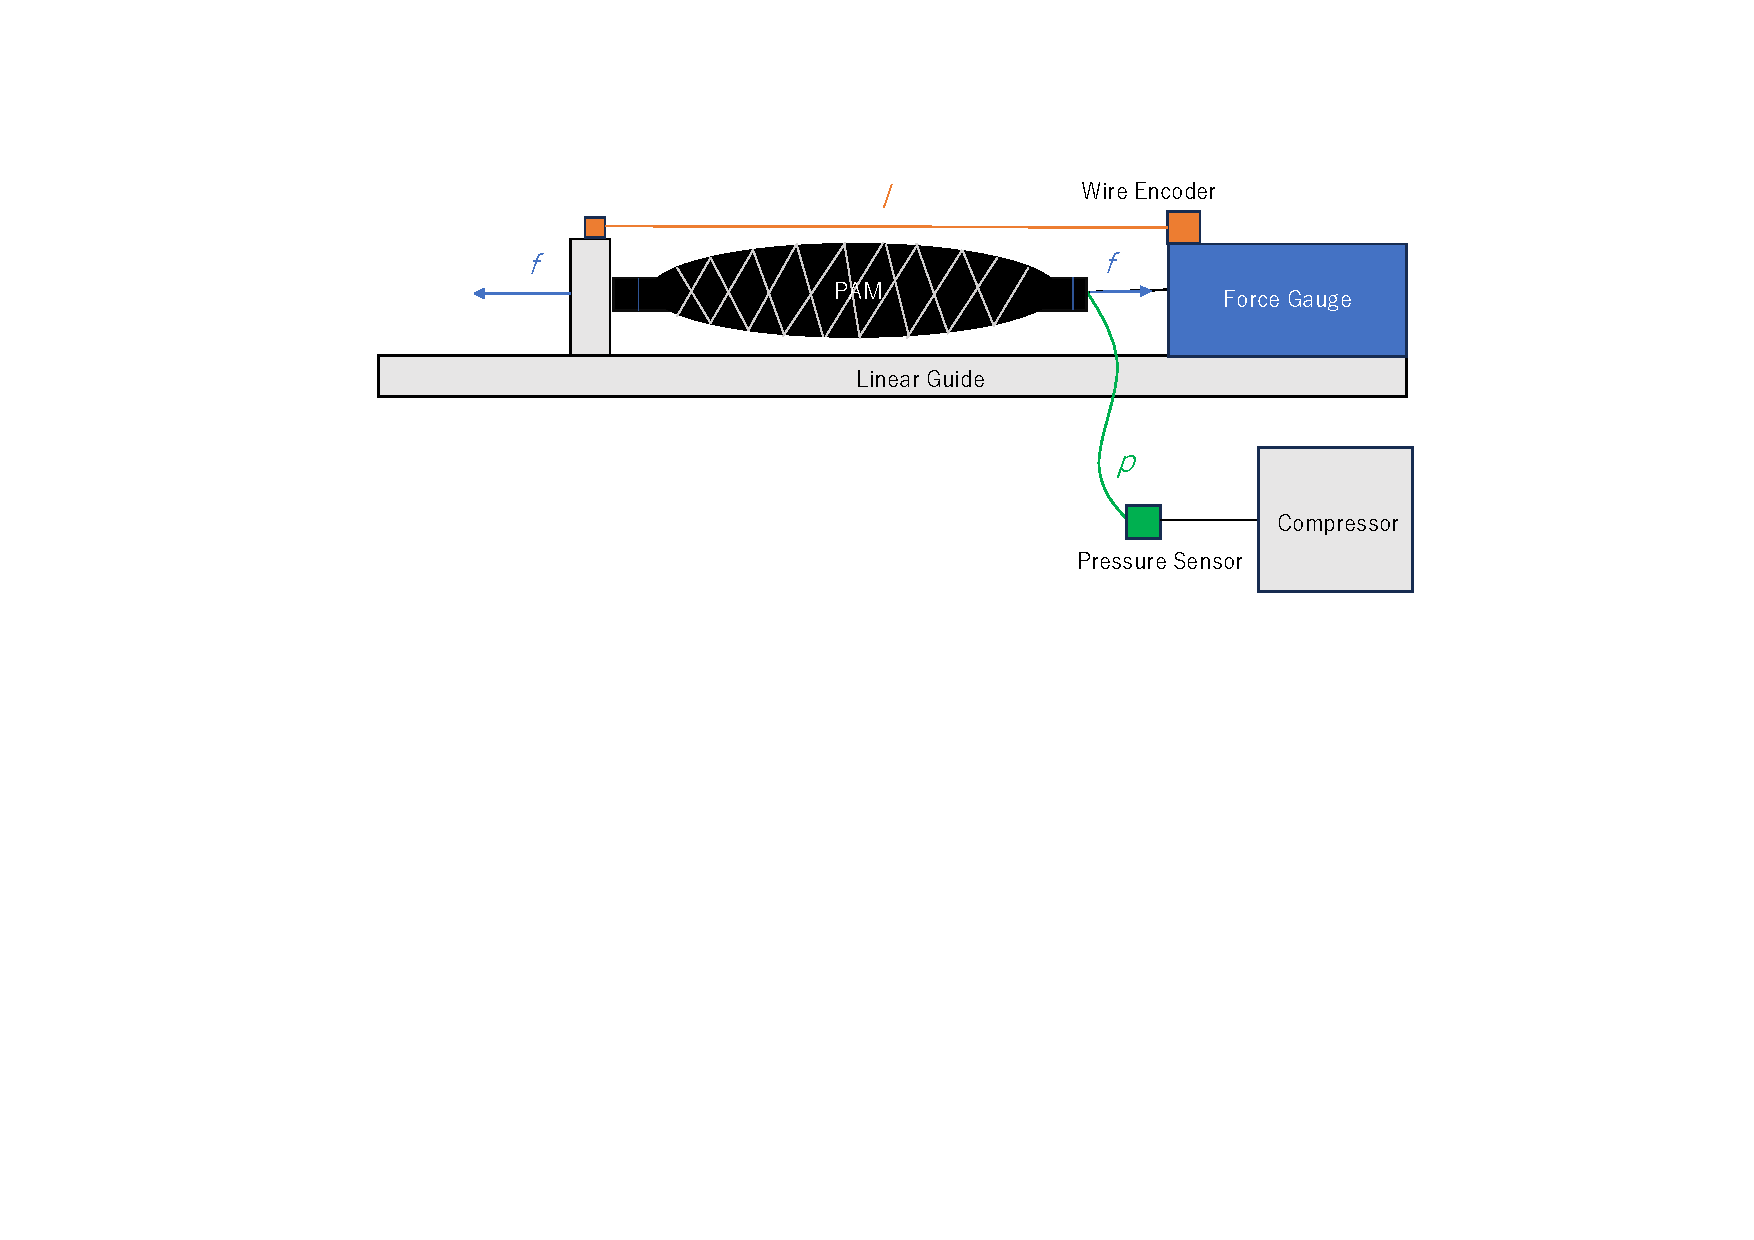
\includegraphics[width=\columnwidth]{fig/static_experiment.pdf}
    \caption{Outline Diagram of Static Tensile Test}
    \label{fig:static_equipment}
 \end{figure}
 \begin{table}[t]
    \centering
    \caption{Characteristics of Experimented PAMs}
    \begin{tabular}{c|ccccc}
        \hline
        PAM & Length [$\si{mm}$] & Diameter [$\si{mm}$] & bladder Material\\
        \hline \hline
        A & 216 & 19.9 &  Rubber \\
        B &211  & 13.4 &  Rubber \\
        C & 141 & 13.4 &  Rubber \\
        D & 212 & 19.0 & Silicone \\
        Agonist & 180 & 16.0 & Rubber \\
        Antagonist & 180 & 16.1 & Rubber \\
        \hline
    \end{tabular}
\label{tab:PAM}
\end{table}

\subsection{Reaching Task}
We conducted reaching experiments to see errors when the model is actually incorporated into a robot arm. The system developed by Takahashi et al.\cite{takahashi} was adapted and positioned vertically. The system consisted of an arm with a pair of PAMs, an agonist muscle and an antagonist, and their shapes and materials are listed in Table \ref{tab:PAM}. The PAMs were connected to the arm with fishing line via shafts, and foil strain gauges (KFP-5-120-C1-65L1M2R, Kyowa Electronic Instrument Co. Ltd.) based on acrylic boards were attached to one end of each PAM. To validate the performance of the model in comparison with a conventional method, we wrapped the PAMs with conductive fiber sensors developed by Hitzmann et al. \cite{fiber}, which assesses the rate of change in length by detecting variations in resistance and thereby calculating the rate of change in diameter.
The reaching movement was achieved by linearly increasing the pressure of the agonist muscle from 0.2 $\si{MPa}$ to 0.6 $\si{MPa}$ while simultaneously decreasing the pressure of the antagonist from 0.6 $\si{MPa}$ to 0.2 $\si{MPa}$. During the reaching movement, the length of the PAM was measured with the linear encoder while it was estimated by the model and the fiber sensor, and the errors were calculated. The experiment time was 12 $\si{s}$, and the sampling frequency was set to 100 $\si{Hz}$.

During the experiment, the change in resistance of the strain gauges went to a quarter Wheatstone bridge circuit where three other resistors were $120 \pm 0.5 \Omega$, and voltage signal from the circuit was converted to force according to Eq. (\ref{eq:voltage}). Eq. (\ref{eq:voltage}) assumes that voltage is a linear function of force because voltage of a Wheatstone bridge circuit is proportional to strain\cite{wheatstone} and strain is proportional to force while material elastically deforms.
\begin{equation}
    \label{eq:voltage}
    V=qf+V_{base}
\end{equation}
$V$ is the voltage signal from the strain gauge, $q$ is the slope of voltage to force, and $V_{base}$ is the voltage when no force is applied.
The parameter $q$ was obtained by measuring voltage and force while statically loading the strain gauge.
Eq.(\ref{eq:voltage}) can be rewritten as
\begin{equation}
    \label{eq:voltage_2}
    f = \frac{1}{q}\Delta V
\end{equation}
where $\Delta V = V - V_{base}$. Substituting Eq. (\ref{eq:voltage_2}) into Eq. (\ref{eq:model}) gives
\begin{equation}
    \label{eq:model_voltage}
    \Delta V = (a'_3pd + a'_2p + a'_1d + a'_0)d
\end{equation}
in which $a'_i=qa_i$, and the deformation $d$ can be calculated by solving this equation.

\subsection{Stretch Reflex}
\begin{figure}[t]
    \centering
    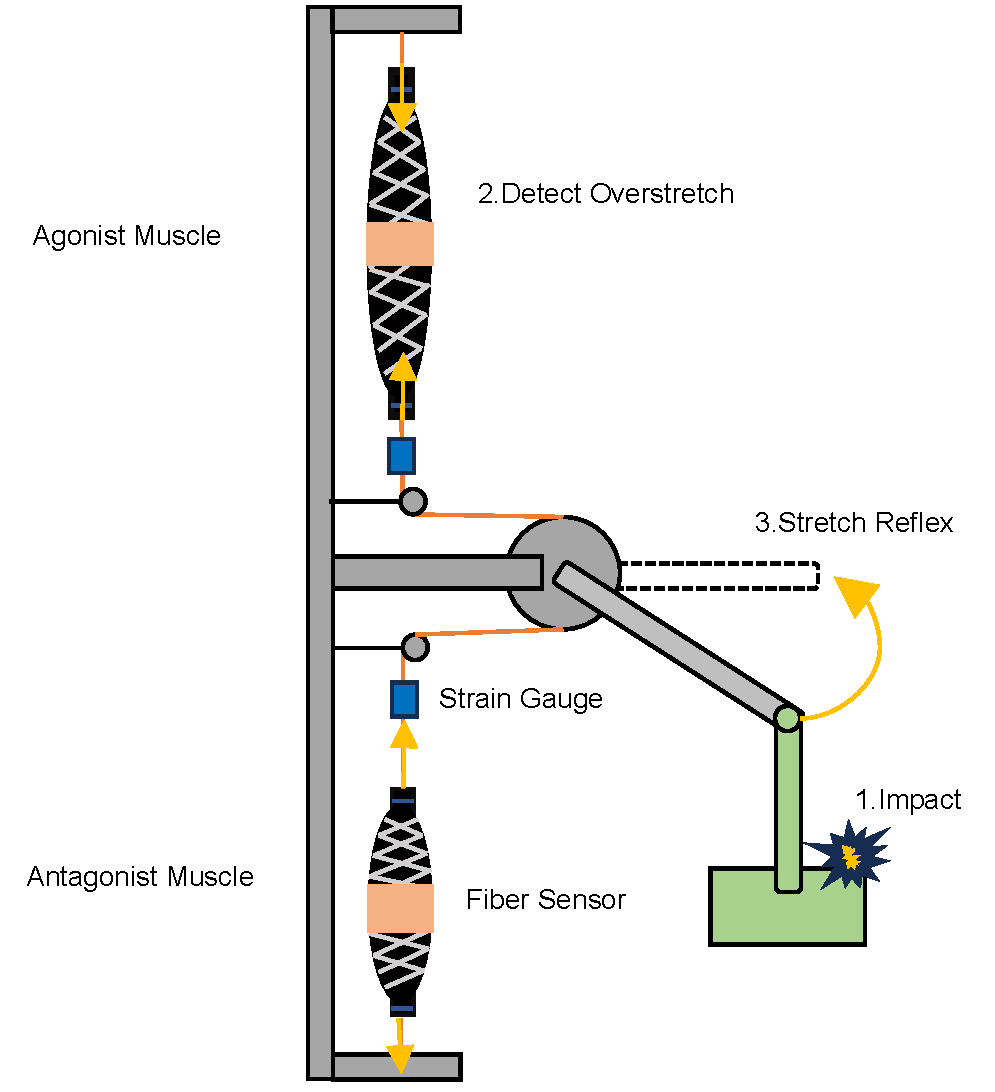
\includegraphics[width=0.7\columnwidth]{fig/reflex_experiment.pdf}
    \caption{Outline Diagram of Stretch Reflex Experiment}
    \label{fig:reflex_equipment}
 \end{figure}
Fig. \ref{fig:reflex_equipment} is an outline diagram of the stretch reflex experiment.
The arm was equipped with the basket and expected to keep it in a fixed position by maintaining the pressure of both PAMs at 0.4 $\si{MPa}$, and a 0.2 $\si{kg}$ mass was dropped from a height of 14 $\si{cm}$ to make an impact. During the experiment, velocities of the PAMs were calculated as
\begin{equation}
    \label{eq:velocity}
    v_j = \frac{l_j -l_{j-1}}{dt}
\end{equation}
where $j$ is the sampling number, $l_j$ is the estimated length, and $dt$ is the sampling period.
Since the system was set to 100 $\si{Hz}$, $dt$ was 0.01 $\si{s}$.
When the impact rapidly stretched the agonist PAM and its velocity exceeded a predetermined threshold, the stretch reflex was induced for 200 $\si{ms}$. The pressure command from the stretch reflex mechanism converged to the goal pressure from a top controller as follows
\begin{align}
    \label{eq:command_pressure}
    p_{ago} &= p_{tp - ago} + \Delta p_{ago - exci} - \Delta p_{anta - inhi} \\
    p_{anta} &= p_{tp - anta} + \Delta p_{anta - exci} - \Delta p_{ago - inhi}
    \label{eq:command_pressure_2}
\end{align}
in which $p_{tp}$ is the goal pressure from the top controller, $\Delta p_{exci}$ is the excitatory pressure from the reflex mechanism, and $ \Delta p_{inhi}$ is the reciprocal inhibition pressure. 
$\Delta p_{exci}$ and $\Delta p_{inhi}$ were calculated by the following equation.
\begin{equation}
    \label{eq:reflex_pressure}
    \Delta p_{exci} =  \Delta p_{inhi} = kv
\end{equation}
The velocity thresholds $V_{thr}$ and the feedback gains $k$ were predetermined experimentally as shown in Table \ref{tab:reflex_para} by assessing magnitude of impact from a falling mass. Takahashi et al. designed the reflex command Eq. (\ref{eq:command_pressure}) and Eq. (\ref{eq:command_pressure_2}) inspired by $\alpha$ motor neurons in human spinal cords \cite{takahashi}. The positioning tasks were conducted applying the stretch reflexes both with the model and the fiber sensor, and the reaction behaviors were compared.


\section{RESULT}
\subsection{Parameter Identification}
Fig. \ref{fig:length_pressure} displays the relationship between the pressure $p$ and the natural length $l_n$ of the PAMs. As assumed, there is a tendency for $l_n$ to decrease linearly with $p$ within the range of the tested pressure. The dashed lines in Fig. \ref{fig:length_pressure} represent the fitted lines using the least squares method, expressed by Eq. (\ref{eq:L_n}).
Fig. \ref{fig:pam_b_static1} shows the result of the static loading experiment for PAM-B. The red and blue points represent the data during expansion and contraction respectively, and the green dashed lines represent the solutions $d$ to Eq. (\ref{eq:model}), which is given by substituting the acquired parameters $a_i$ and the measured $f$ and $p$.
Generally, PAMs exhibit hysteresis due to friction, so the data differ between expansion and contraction processes. We only present the static loading experimental result for PAM-B because of the space constraint, but similar results were obtained for the other PAMs.

\begin{figure}[t]
    \hfill
    \begin{minipage}{\columnwidth}
        \centering
        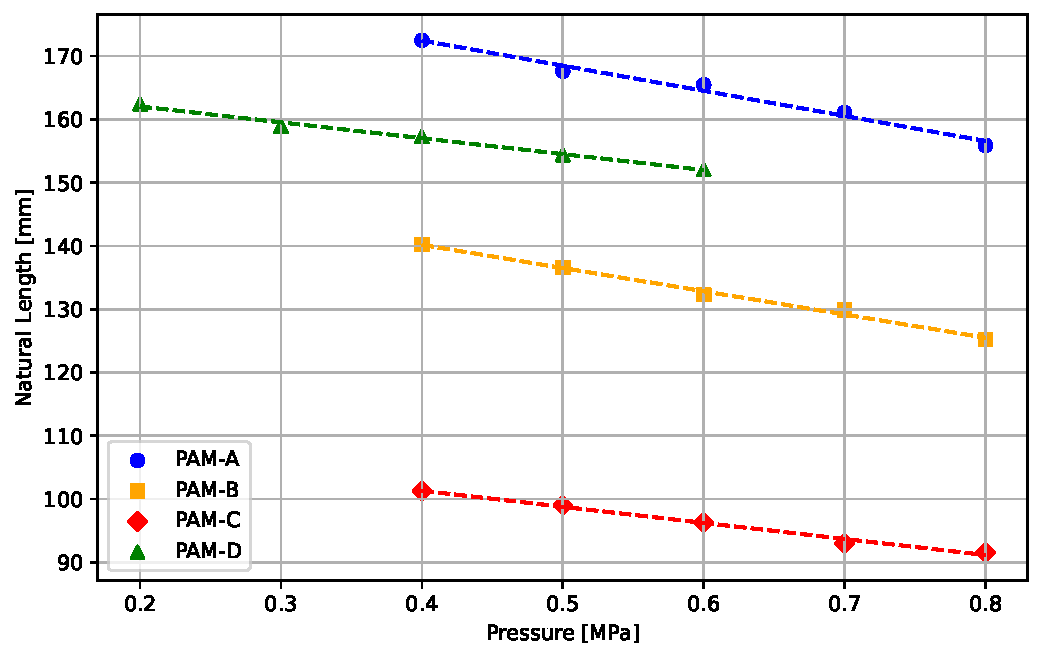
\includegraphics[width=\columnwidth]{fig/length_pressure.pdf} 
        \caption{Relationship between Pressure and Natural Length}
        \label{fig:length_pressure}
        \vspace{1em} 
        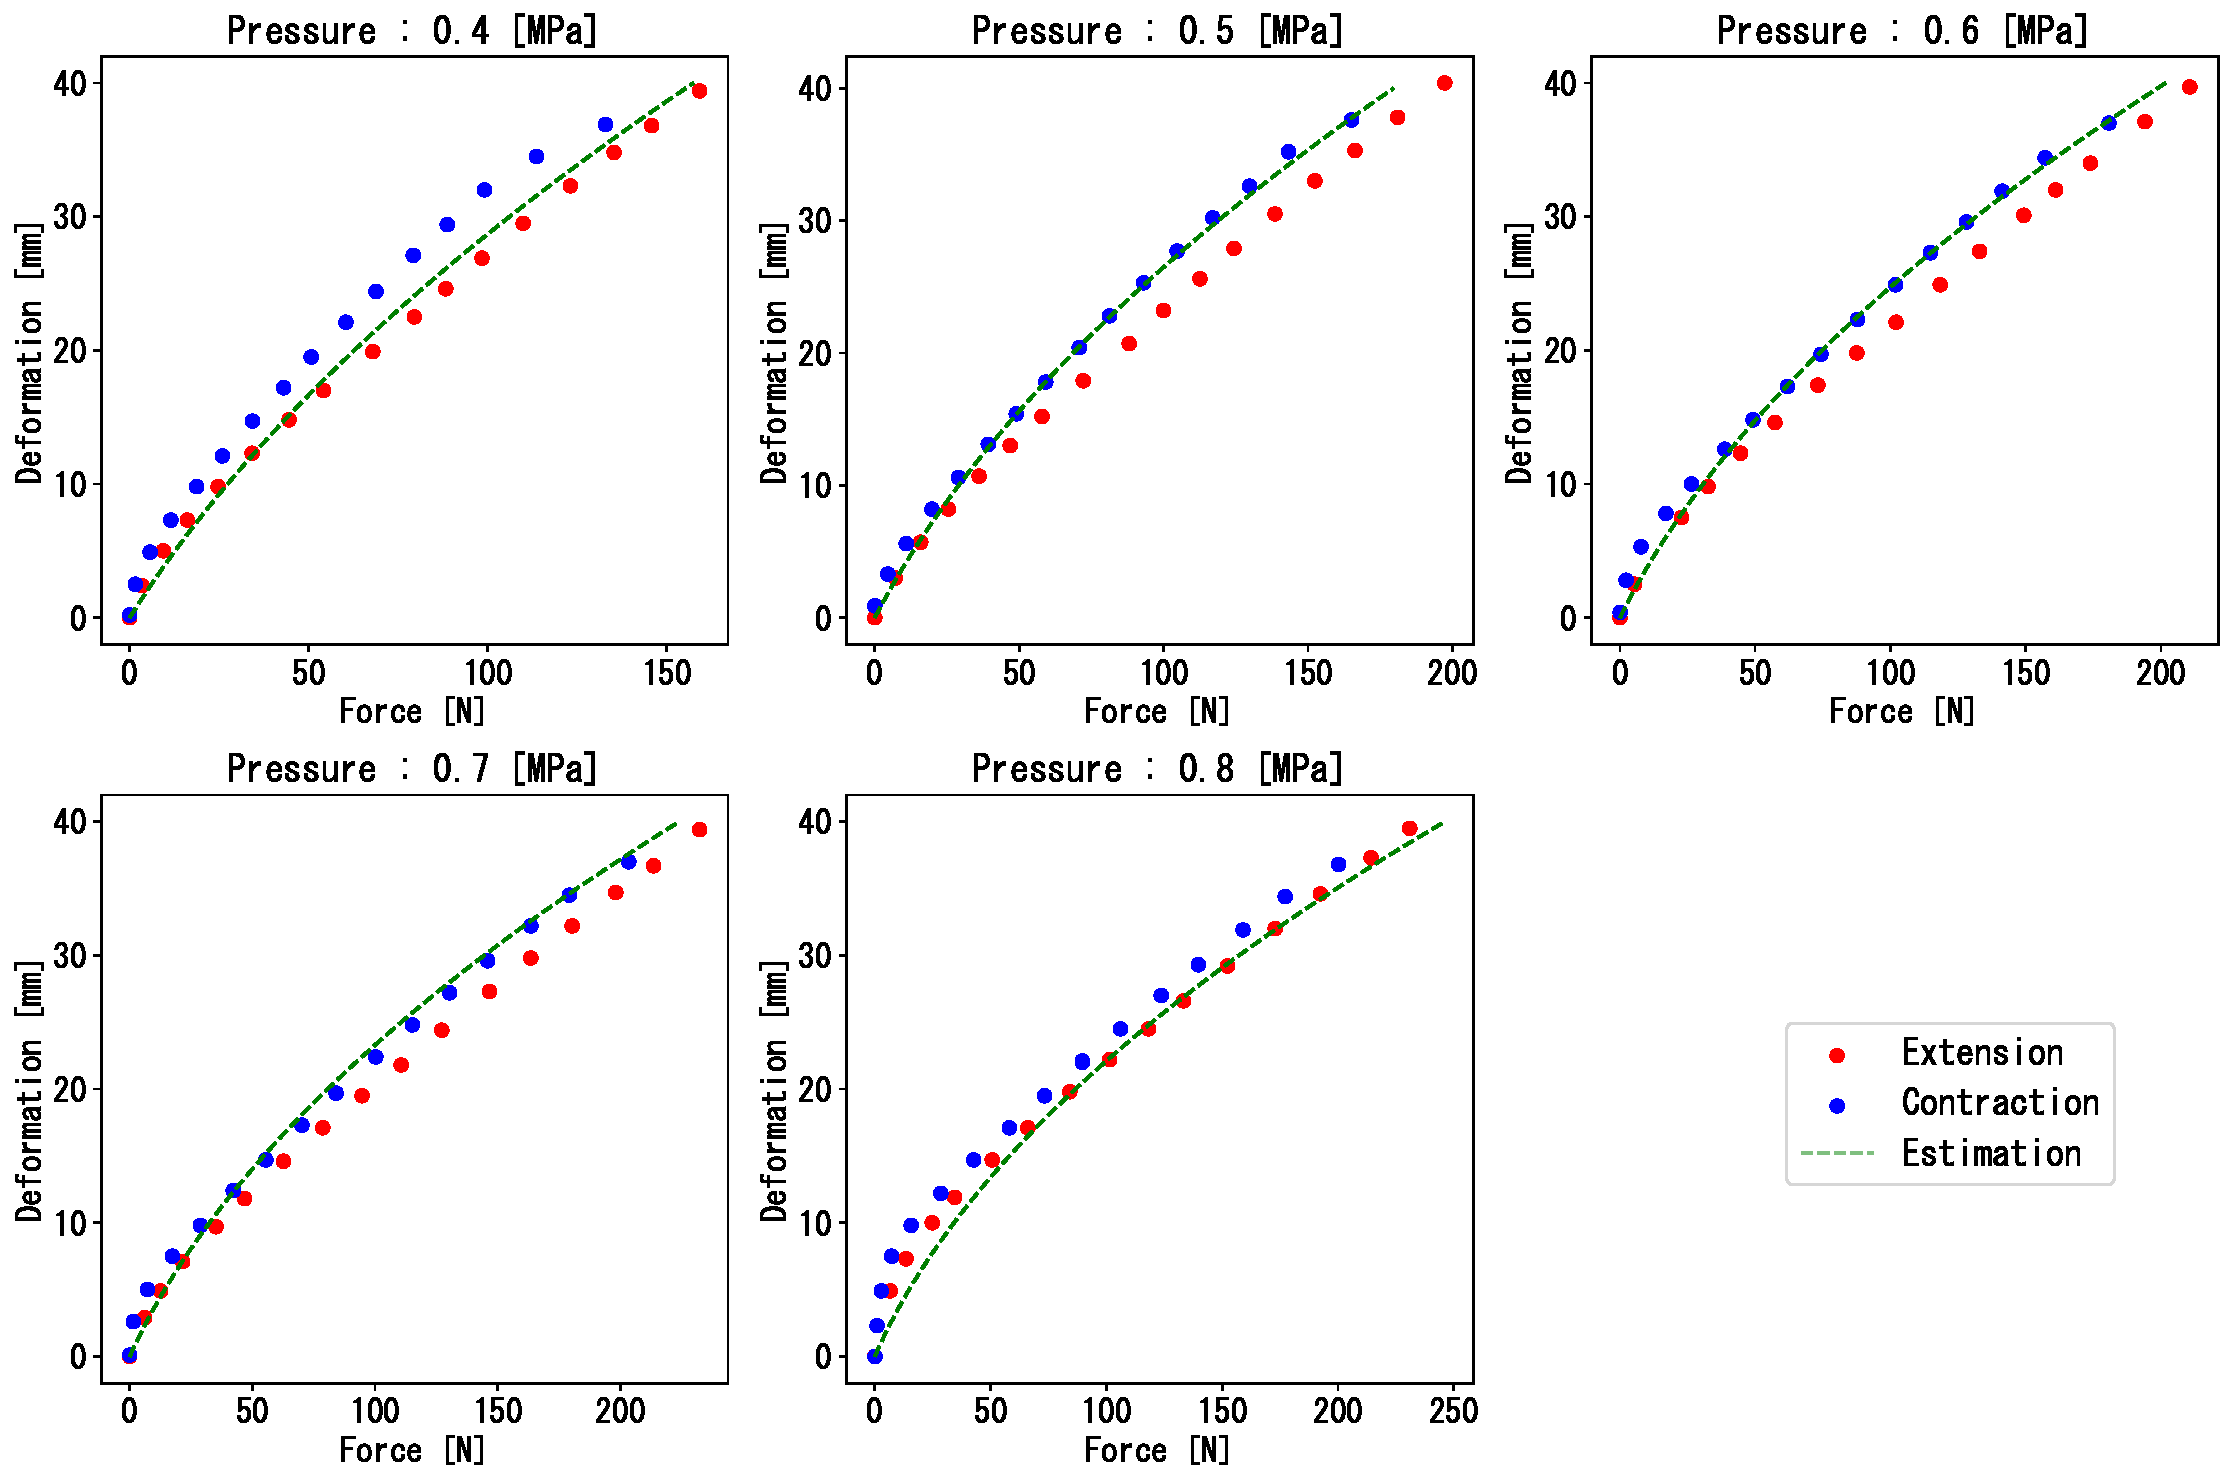
\includegraphics[width=\columnwidth]{fig/20231124_5_4s_2d_ieeesensors1.pdf}
        \caption{Relationship between Force and Deformation at Each Pressure (PAM-B)}
        \label{fig:pam_b_static1}
    \end{minipage}
    \hspace{0.05\textwidth} 
\end{figure}




% \begin{textblock*}{\columnwidth}(11cm,3cm) 
% \begin{figure}
%     \centering
%     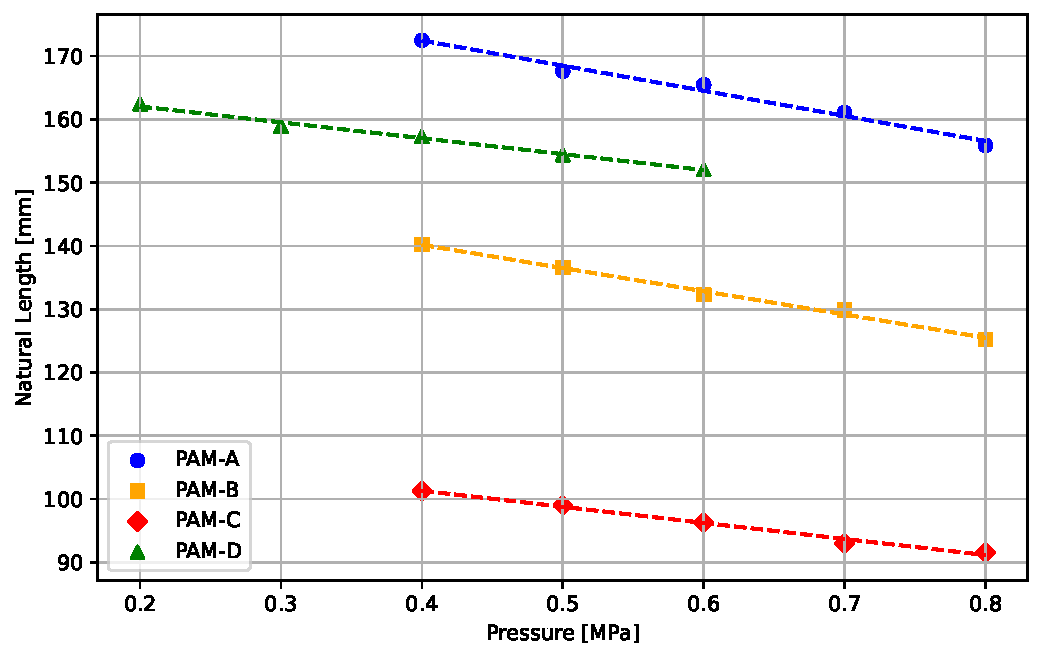
\includegraphics[width=\columnwidth]{fig/length_pressure.pdf}
%     \caption{Relationship between Pressure and Natural Length}
%     \label{fig:length_pressure}
% \end{figure}
% \end{textblock*}


% \begin{textblock*}{\columnwidth}(11cm,12cm) 
% \begin{figure}
%    \centering
%    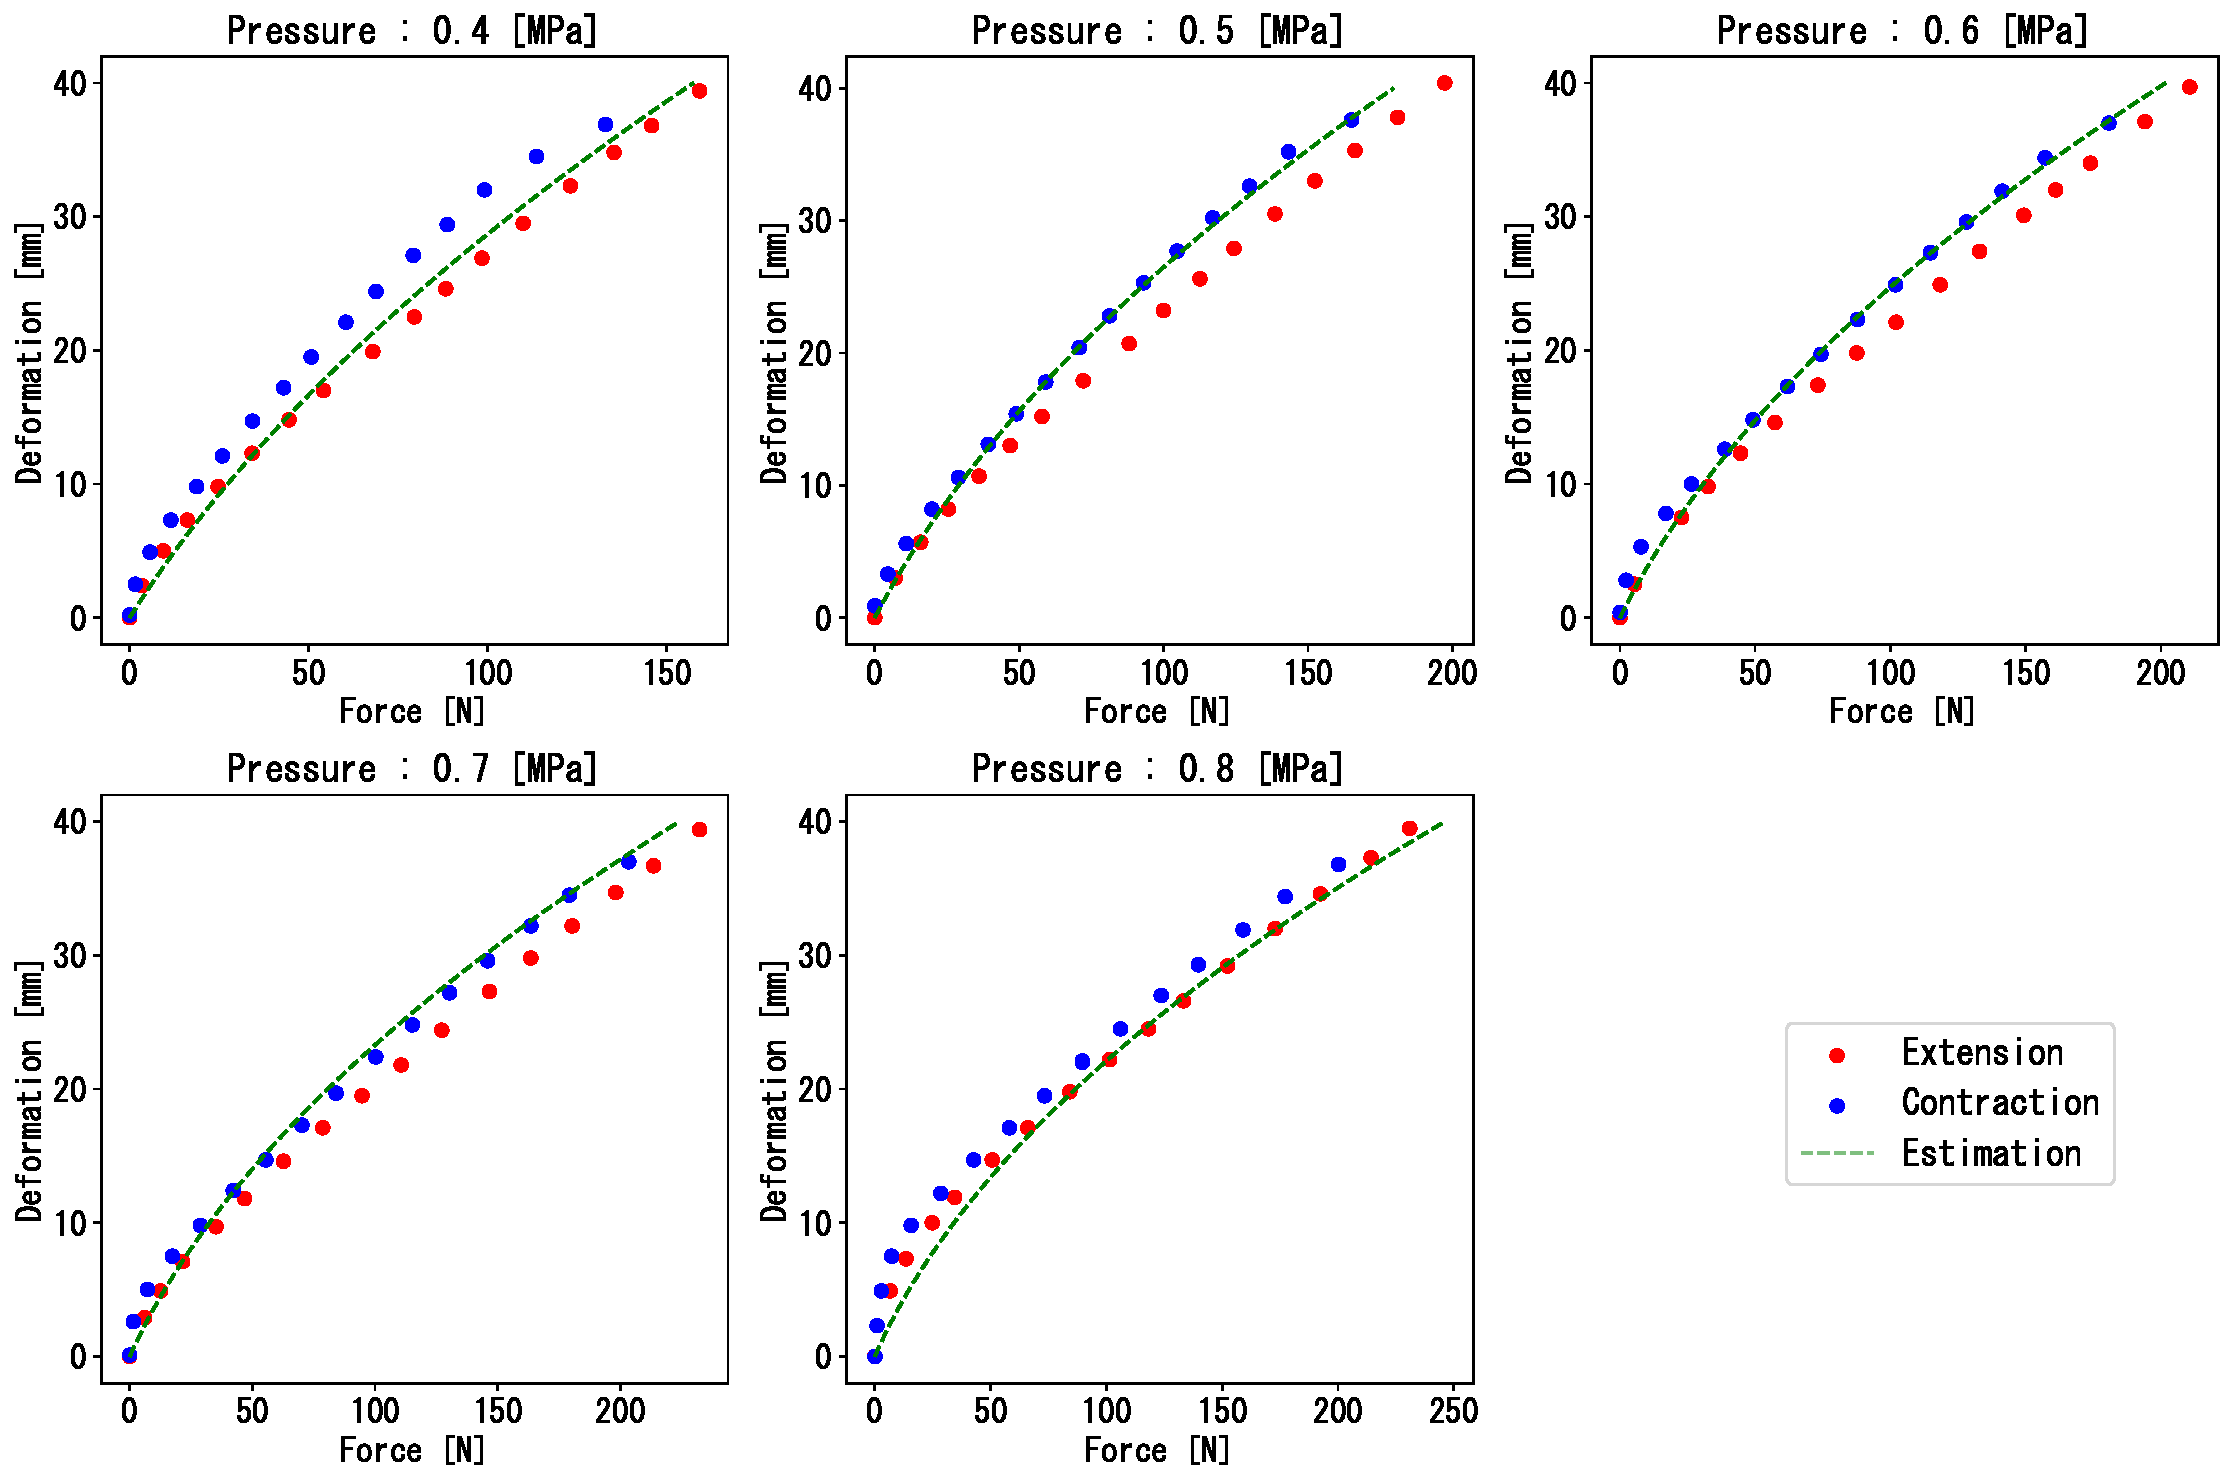
\includegraphics[width=\columnwidth]{fig/20231124_5_4s_2d_ieeesensors1.pdf}
%    \caption{Relationship between Force and Deformation at Each Pressure (PAM-B)}
%    \label{fig:pam_b_static1}
% \end{figure}
% \end{textblock*}

% % 画像にかからないようにテキスト位置を調整
% \vspace{40cm} % 必要に応じて調整してください

% \begin{figure}[H]
%     \centering
%     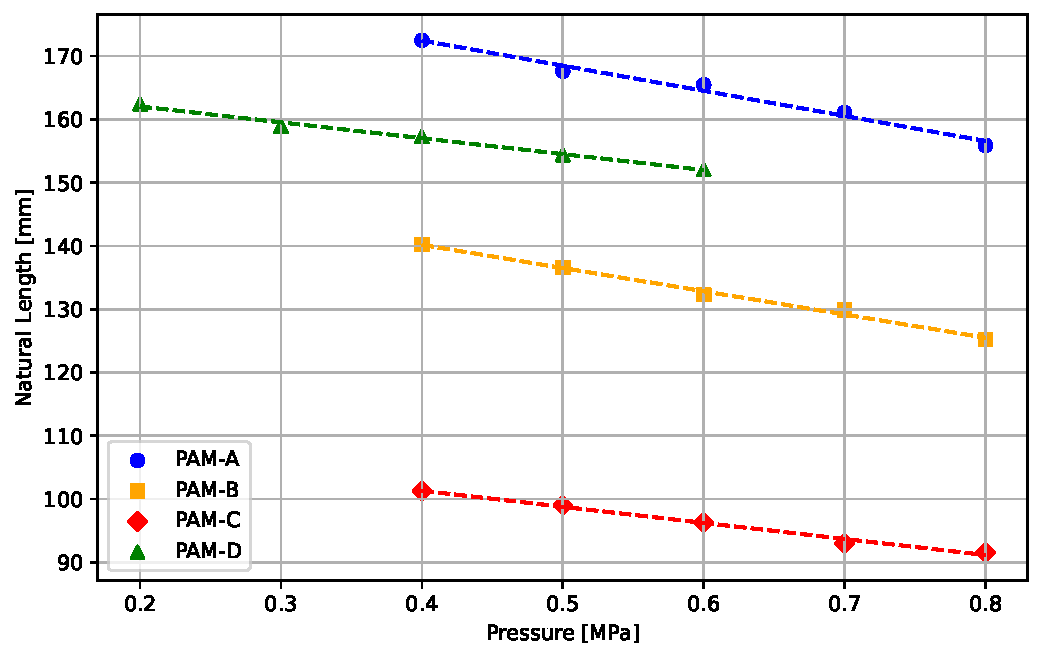
\includegraphics[width=\columnwidth]{fig/length_pressure.pdf}
%     \caption{Relationship between Pressure and Natural Length}
%     \label{fig:length_pressure}
% \end{figure}

% \begin{figure}[H]
%    \centering
%    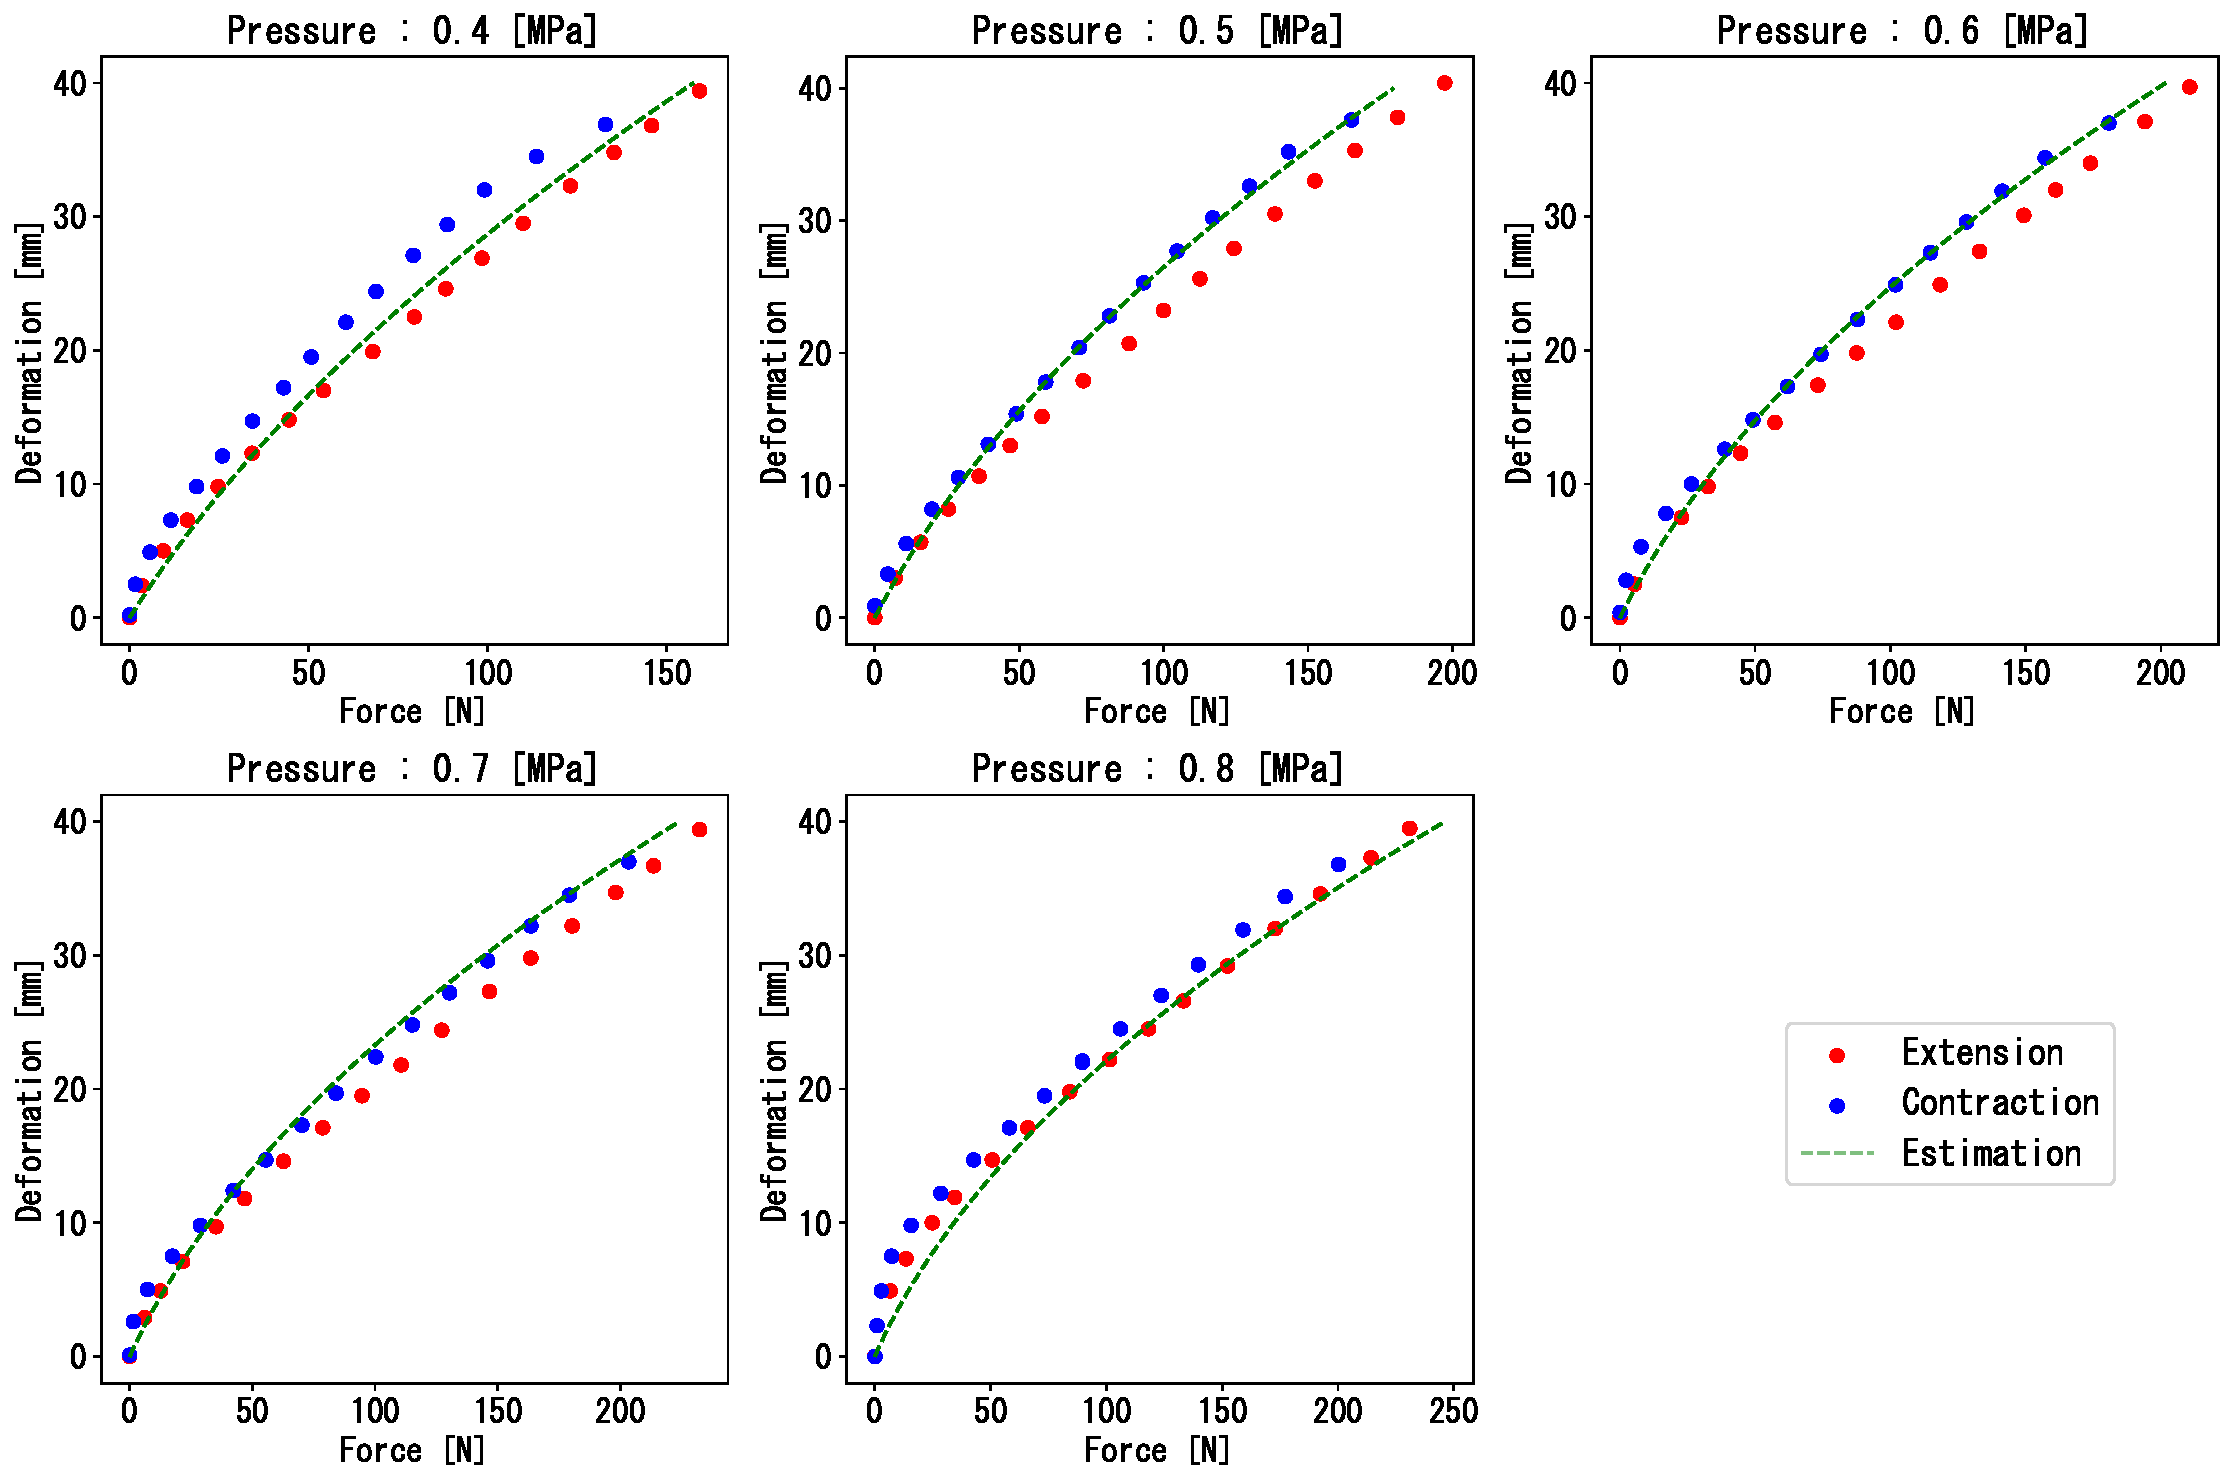
\includegraphics[width=\columnwidth]{fig/20231124_5_4s_2d_ieeesensors1.pdf}
%    \caption{Relationship between Force and Deformation at Each Pressure (PAM-B)}
%    \label{fig:pam_b_static1}
% \end{figure}


\begin{figure*}[h]
   \begin{center}
       \begin{minipage}[t]{\columnwidth} 
           \centering
           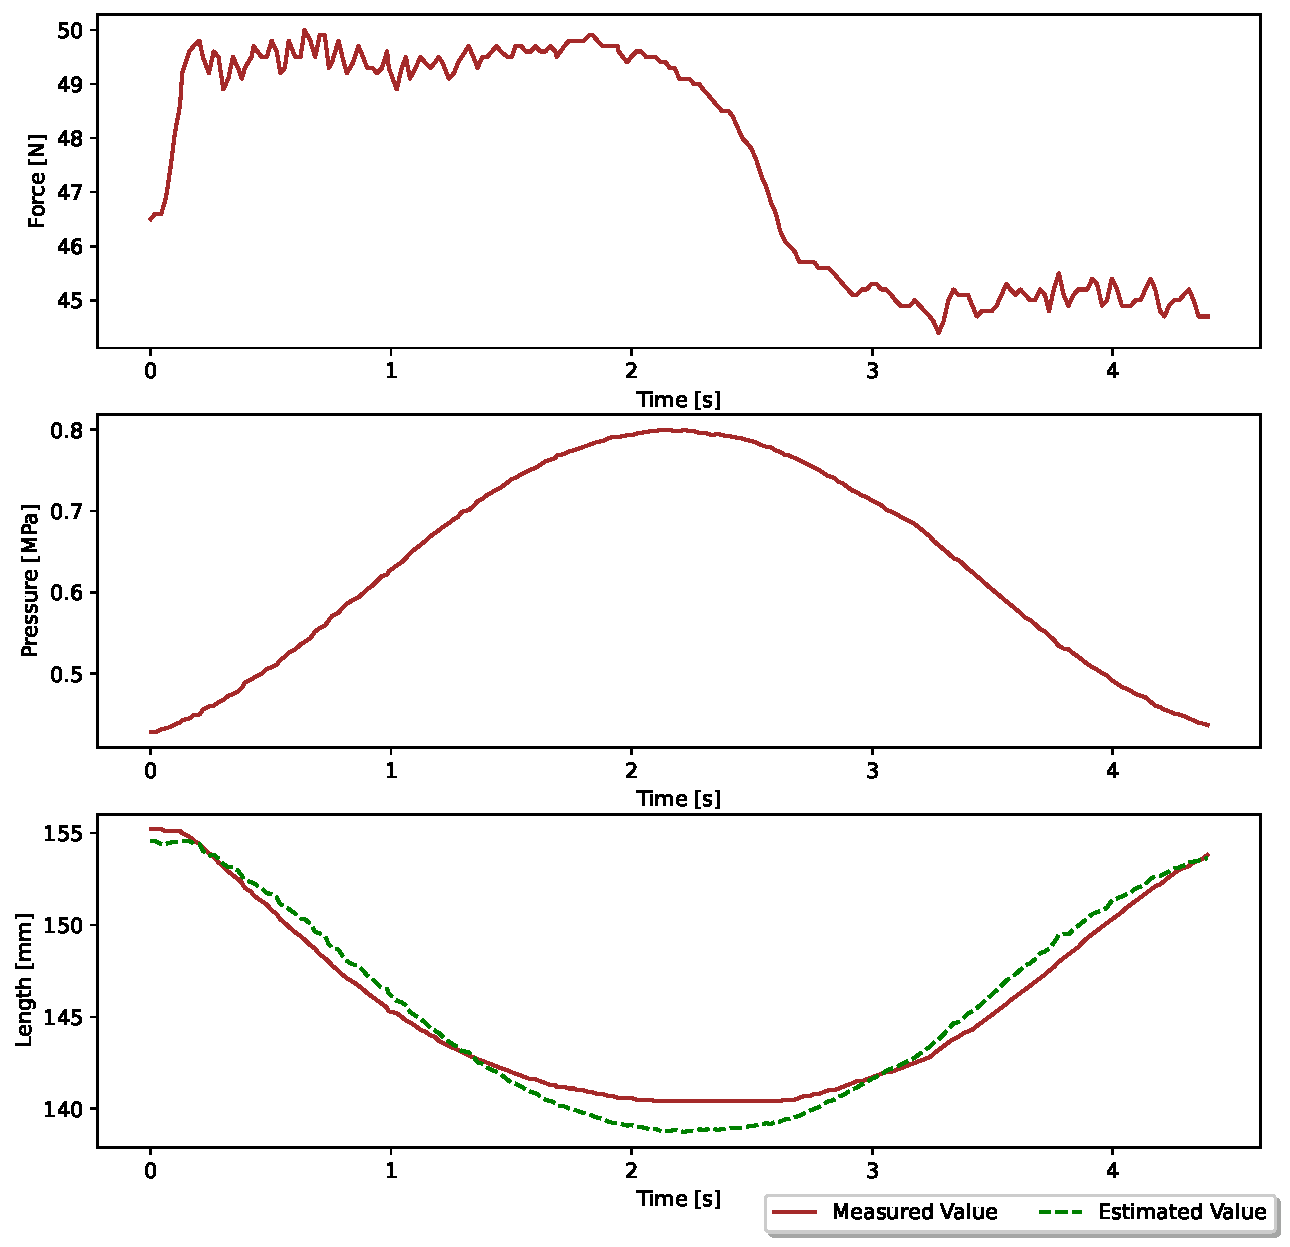
\includegraphics[keepaspectratio, width=\columnwidth]{fig/20231207_1_4s_by_5_2d_ieeesensors1.pdf}
           \caption{Dynamic Length Estimation (PAM-B, Rubber)}
           \label{fig:pam_b_dynamic}
       \end{minipage}
       \hfill
       \begin{minipage}[t]{\columnwidth} 
           \centering
           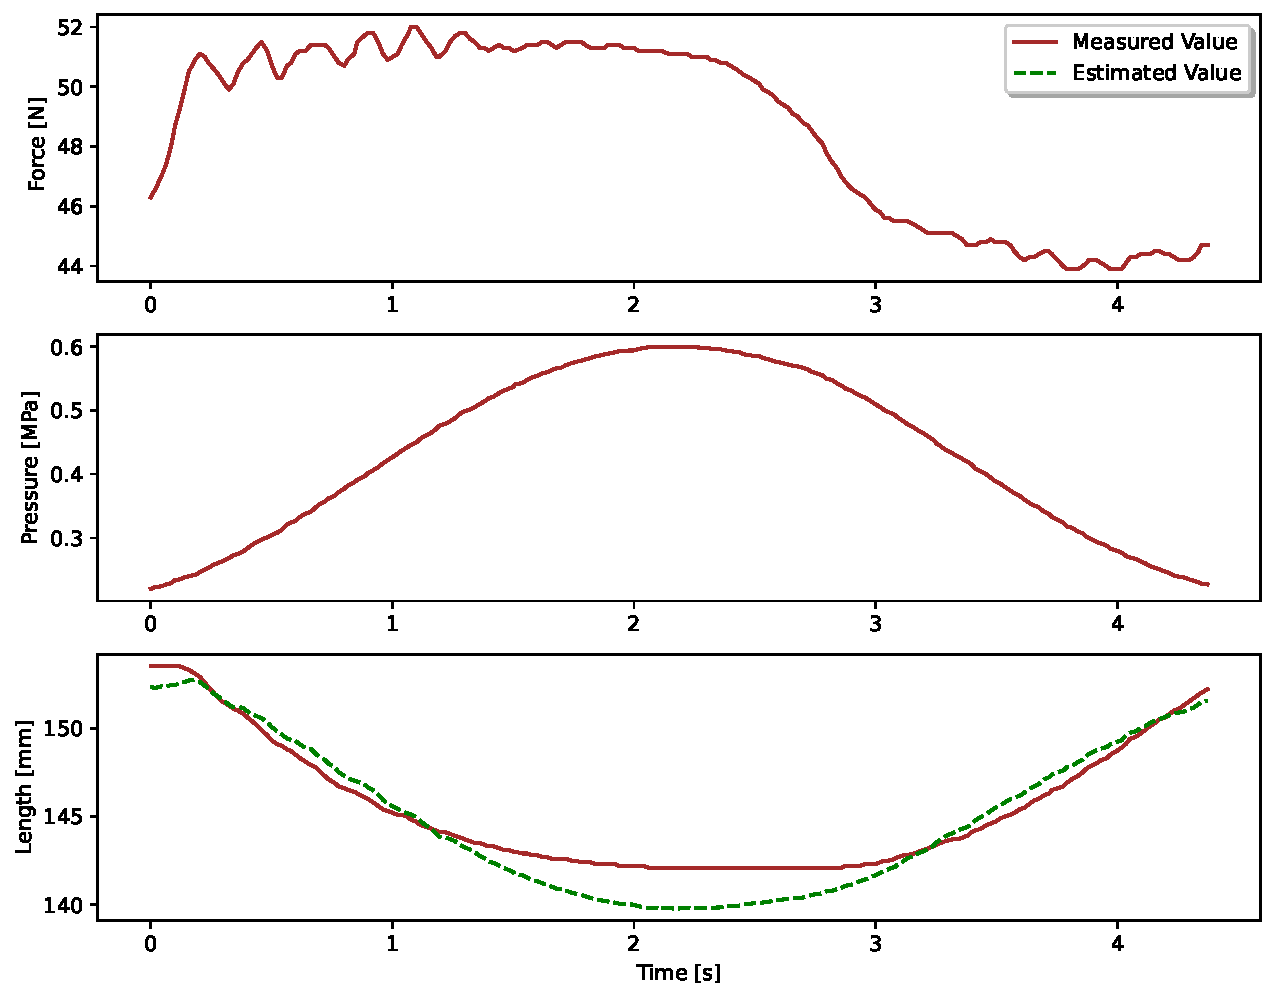
\includegraphics[keepaspectratio, width=\columnwidth]{fig/20231220_2_s_by_2_2d_ieeesensors1.pdf}
           \caption{Dynamic Length Estimation (PAM-D, Silicon)}
           \label{fig:pam_d_dynamic}
       \end{minipage}
   \end{center}
\end{figure*}

\vspace{1cm}

% \begin{figure}[H]
%    \centering
%    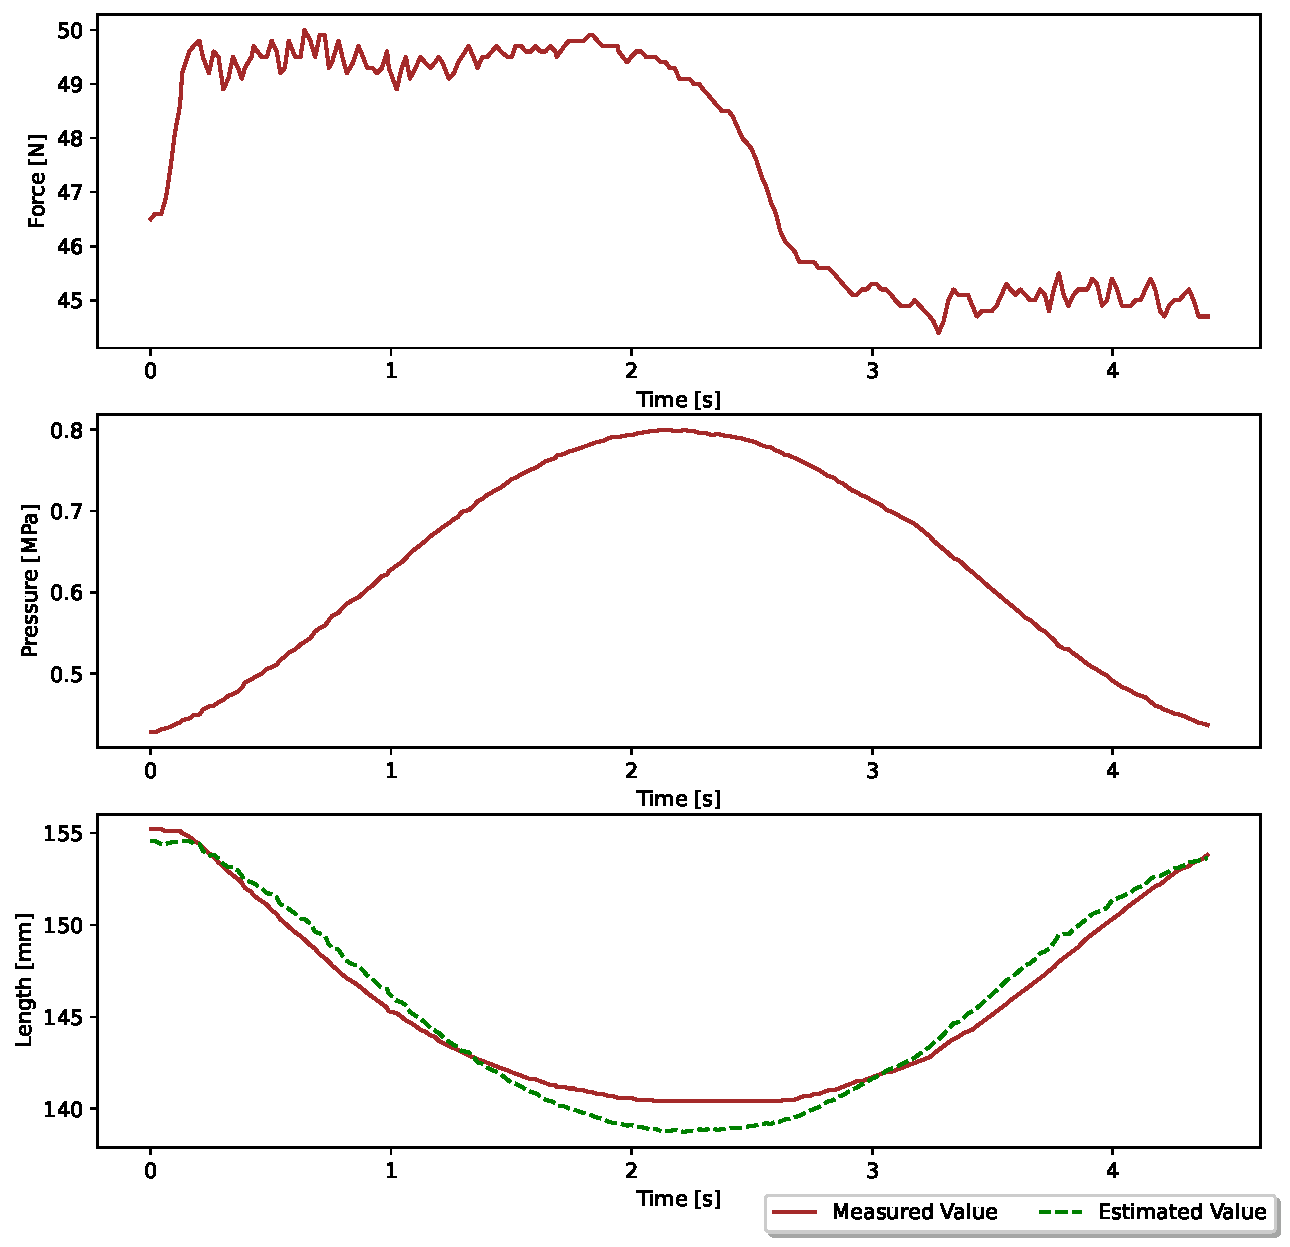
\includegraphics[width=\columnwidth]{fig/20231207_1_4s_by_5_2d_ieeesensors1.pdf}
%    \caption{Dynamic length estimation (PAM-B, Rubber)}
%    \label{fig:pam_b_dynamic}
% \end{figure}
\subsection{Error Evaluation} 
Fig. \ref{fig:pam_b_dynamic} and Fig. \ref{fig:pam_d_dynamic} show the dynamic length estimation result for PAM-B and PAM-D, respectively.
With the proposed method, with respect to the measurements by the linear encoder, the length estimation was achieved with maximum errors of $1.72\%$ for PAM-A, $1.19\%$ for PAM-B, $1.18\%$ for PAM-B, and  $1.65\%$ for PAM-D respectively , and with root mean squared errors of $0.861\%$ for PAM-A, $0.653\%$ for PAM-B, $0.683\%$ for PAM-C, and $0.846\%$ for PAM-D respectively.

\subsection{Reaching Task}
Table. \ref{tab:PAM_reflex} shows the parameters for the length estimation of the agonist and antagonist muscles. The considerable difference in the voltage-force slope $q$ between the two PAMs is attributable to the varying sensitivities of the handmade strain gauges.

Fig.\ref{fig:reaching_error} displays the length estimation errors of the model and the fiber sensor in reaching task. Since the fiber sensor could only measure the rate of length change and not the absolute length, the estimated absolute length by the fiber sensor was calibrated to the measurement value from the linear encoder at the start of the reaching task. Therefore, it cannot be said that Fig.\ref{fig:reaching_error} is exactly comparing the estimates from the model and from the fiber sensor, but it serves as a reference for examining the accuracy of the model against the conventional sensor. The reaching task was performed five times for both the agonist and antagonist muscles. For the agonist muscle, with respect to the linear encoder measurement, the model showed a maximum error of $5.86\%$ and a root mean squared error of $3.17\%$, while the fiber sensor showed a maximum error of $2.53\%$ and a root mean squared error of $1.02\%$. For the antagonist muscle, the model showed a maximum error of $5.86\%$ and a root mean squared error of $5.02\%$, while the fiber sensor showed a maximum error of $2.53\%$ and a root mean squared error of $1.78\%$. 

\begin{table}[H]
    \centering
    \caption{Parameters for Length Estimation} 
    \resizebox{\columnwidth}{!}{%
    \begin{tabular}{c|ccccccc}
        \hline
        PAM & $m$ & $h$ & $a_3$ & $a_2$ & $a_1$ & $a_0$ & $q$ \\
        \hline \hline
        Agonist & -60.1 & 170.1 & -0.201 & 7.00 & 0.256 & 0.911 & $2.25 \times 10^{-3}$\\
        Antagonist & -70.3 & 178.5 & 0.871 & 1.24 & -0.129 & 22.4 & $4.33 \times 10^{-3}$ \\
        \hline
    \end{tabular}
    } 
    \label{tab:PAM_reflex}
\end{table}

\begin{figure*}[t]
    \centering
    \begin{minipage}[H]{\textwidth} 
        \begin{minipage}[H]{0.48\textwidth} 
            \centering
            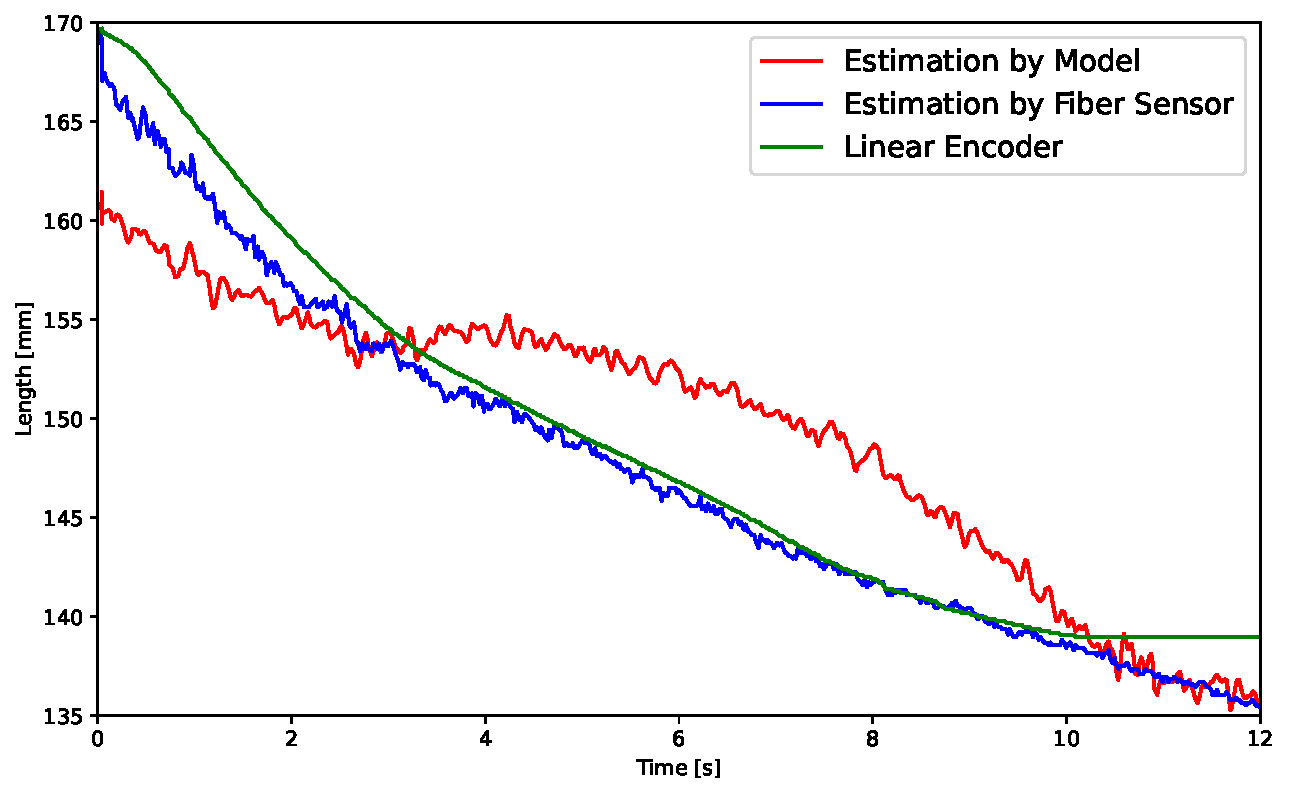
\includegraphics[width=\columnwidth]{fig/reaching_error.pdf}
            \caption{Length Estimation Error in Reaching Task}
            \label{fig:reaching_error}
            \vspace{1em}
            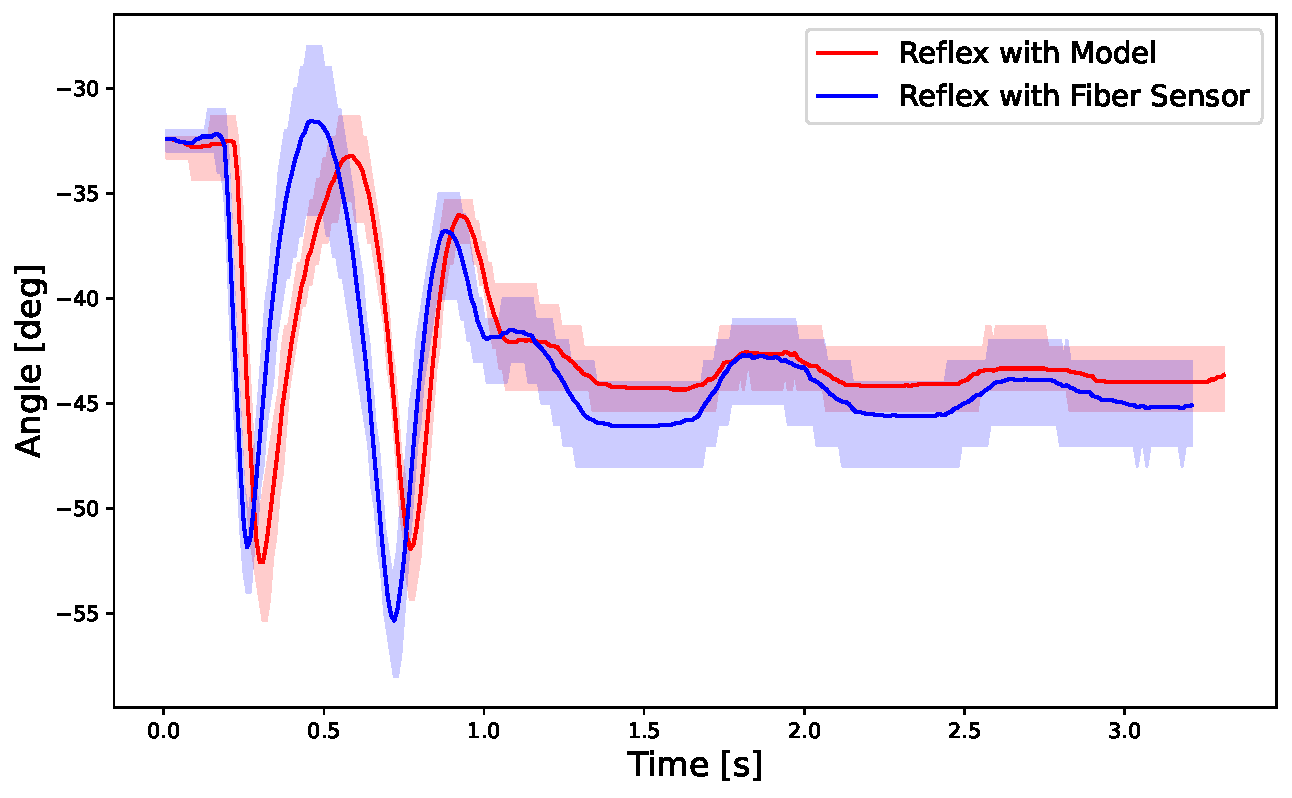
\includegraphics[width=\columnwidth]{fig/time_vs_angle_model_sensor.pdf}
            \caption{Comparison of Reflex Angles between Model and Fiber Sensor}
            \label{fig:reflex_angle}
        \end{minipage}
        \hfill
        \begin{minipage}[H]{0.48\textwidth} 
            \centering
            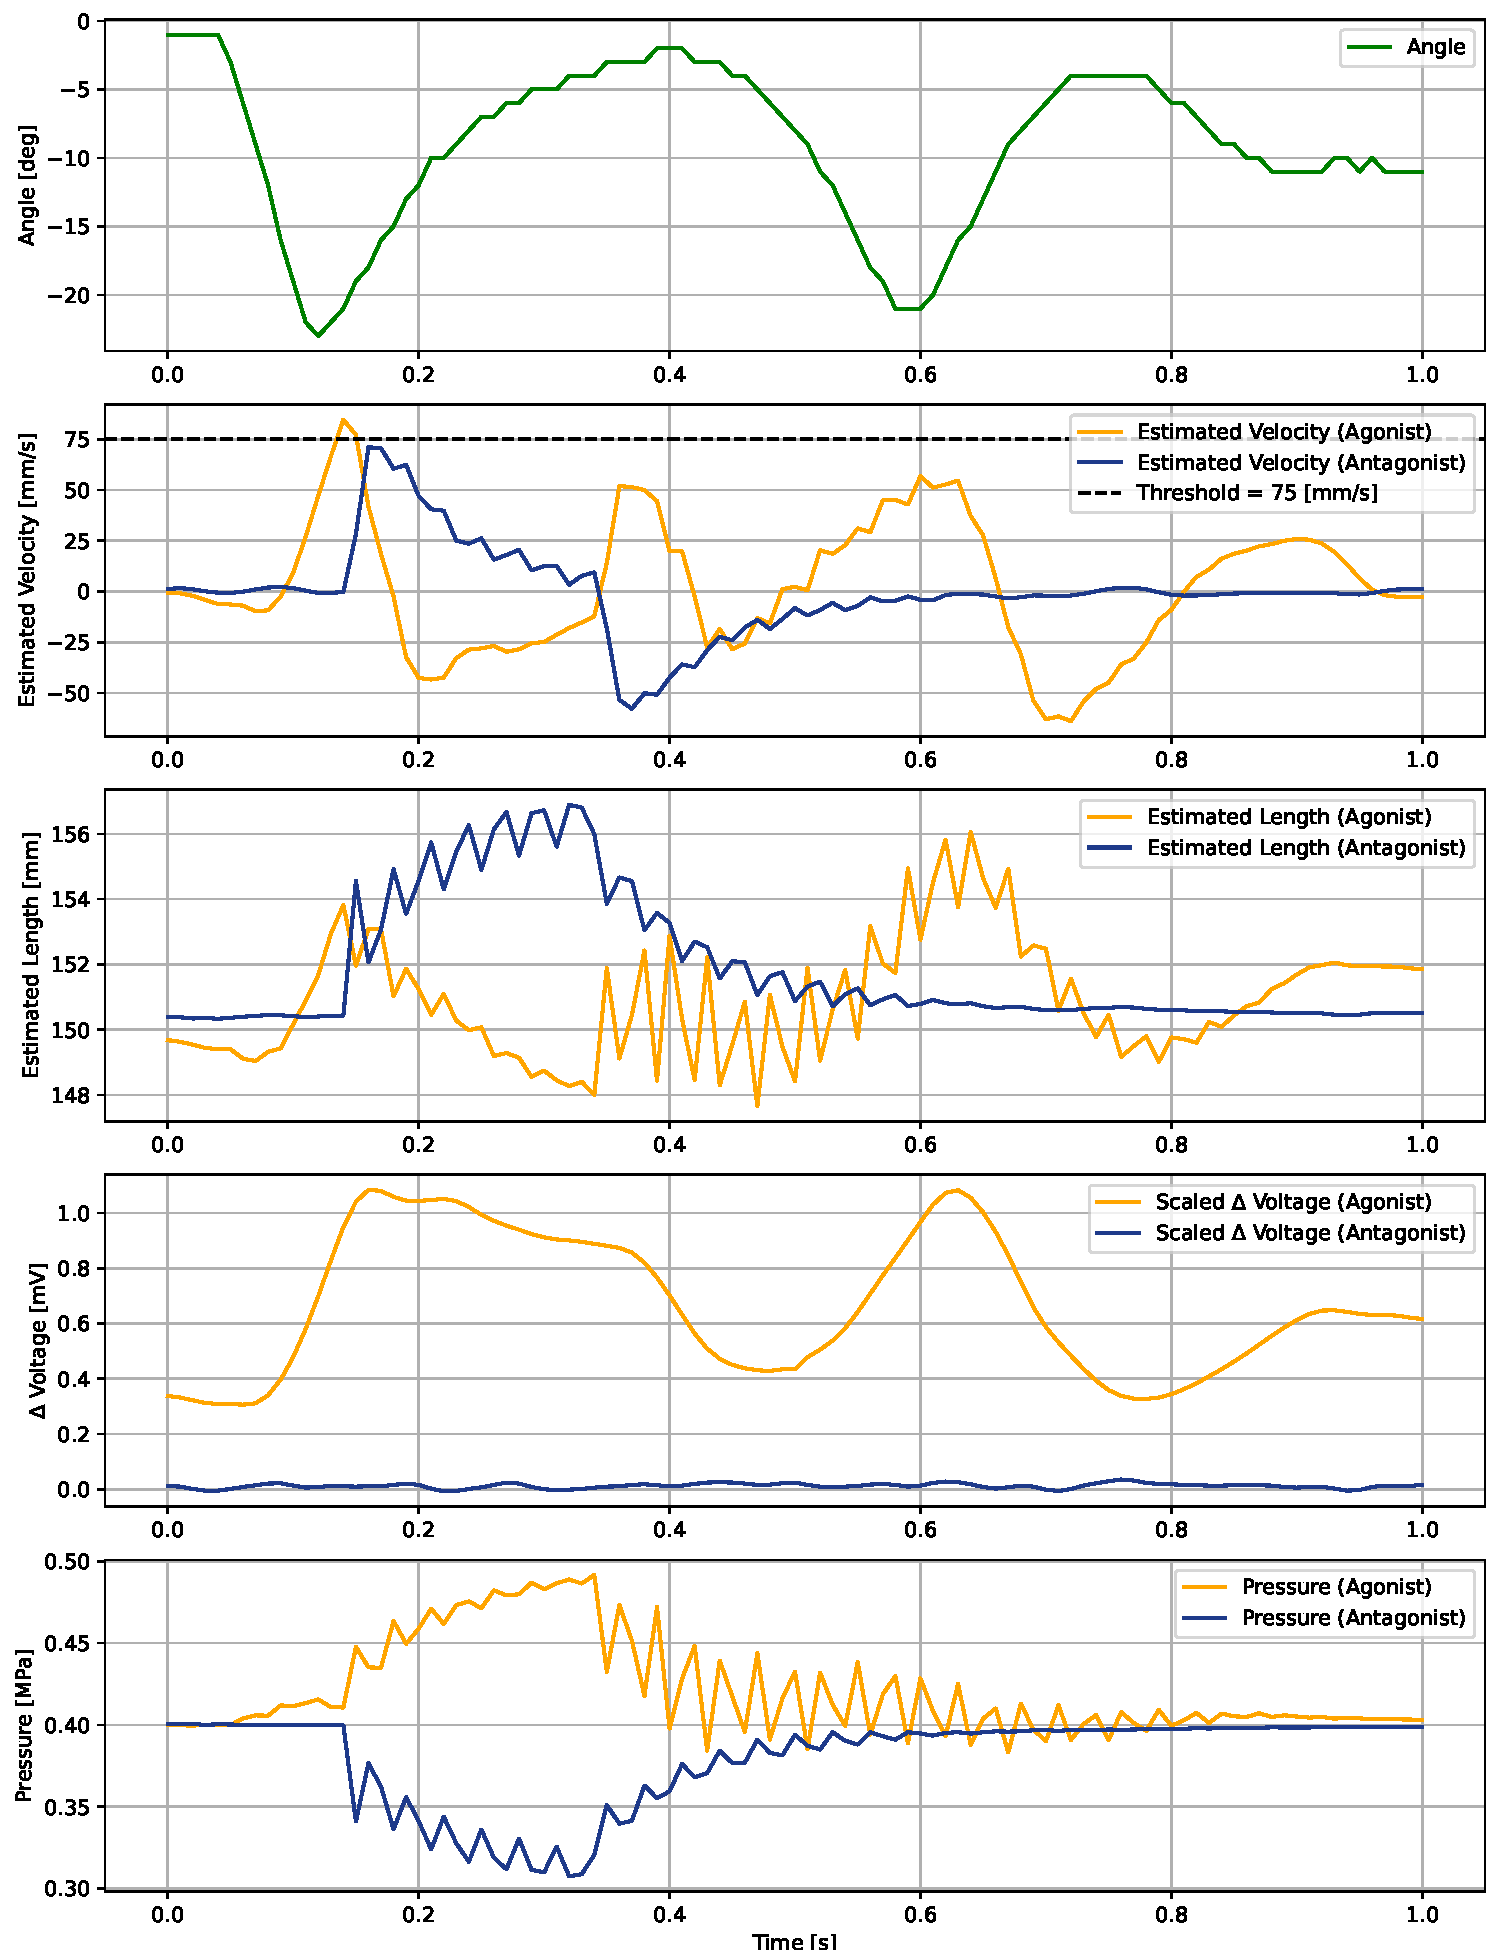
\includegraphics[width=\columnwidth]{fig/20240819_r20_reflex_all_plt.pdf}
            \caption{Dynamic Behavior of Reflex by Model}
            \label{fig:reflex_all}
        \end{minipage}
    \end{minipage}
\end{figure*}
\subsection{Stretch Reflex}
Table \ref{tab:reflex_para} shows the velocity threshold $V_{thr}$ and the feedback gain $k$, and they were determined experimentally by assessing the magnitude of the impact. 

\begin{table}[h]
    \centering
    \caption{Parameters for Stretch Reflex} 
    \begin{tabular}{c|cc}
        \hline
        PAM &$V_{thr} [\si{mm/s}]$&$ k [\si{GPa\cdot s}]$\\
        \hline \hline
        Model & 70 & 1/800\\
        Fiber Sensor & 25 & 1/300\\
        \hline
    \end{tabular}
\label{tab:reflex_para}
\end{table}

Fig. \ref{fig:reflex_all} illustrates the dynamic behavior of the reflex by the model. The starting angle of the arm was -36 deg due to the basket's weight of 83.1 g. When the falling mass made an impact, the angle dropped dramatically, creating sudden soar in the voltage signal from the strain gauge and thus in the estimated velocity. It went beyond the threshold and triggered the stretch reflex, leading to increasing pressure in the agonist muscle and decreasing in antagonist. The arm was then lifted back to the initial position, and after some oscillation, it settled down to a certain angle, holding the mass left in the basket.


Fig.\ref{fig:reflex_angle} displays the average and range of angles in 20 trials of the reflexes by the model and by the fiber sensor. Since the thresholds and gains for each reflex are determined experimentally, it is not possible to purely compare the behavior of the arm angles, but it can be said that the reflex by the fiber sensor are well replicated by the model.




\section{DISCUSSION}
\subsection{Error Evaluation}
To improve length estimation accuracy, we expanded Eq. (\ref{eq:model}) by adding the terms $p^2$ and $d^2$ and increasing the parameters as follows:
\begin{equation}
\label{eq:model_2d(1)}
F = (b_5p^2 + b_4pd + b_3d^2 + b_2p+b_1d+b_0)d
\end{equation}
As a result, with respect to the measurements by the linear encoder,the dynamic length estimation was achieved with the maximum errors of $1.12\%$ for PAM-A, $0.773\%$ for PAM-B, $1.01\%$ for PAM-B, and $0.755\%$ for PAM-D respectively, and with the root mean squared errors of $0.633\%$ for PAM-A, $0.353\%$ for PAM-B, $0.548\%$ for PAM-C, and $0.435\%$ for PAM-D respectively. The errors were reduced as expected for all PAMs. 
% As a result, the dynamic length estimation was achieved with maximum errors within $1.12\%$ and mean squared error rates within $0.633\%$, and the errors were reduced as expected for all PAMs. 

% As a result, as shown in the third and fourth columns of Table \ref{tab:error}, the errors were reduced as expected for all PAMs. 

We also tried another approach by introducing a cubic polynomial model and increasing the parameters as follows:
\begin{equation}
    \label{eq:model_3d}
    F = (c_4p^3+c_3p^2d+c_2pd^2+c_1d^2+c_0)d
\end{equation}
As predicted, the root mean squared errors decreased to $0.516\%$ for PAM-A, $0.484\%$ for PAM-B, $0.500\%$ for PAM-C, and $0.606\%$ for PAM-D respectively. 
However, even though the maximum errors decreased to $1.22\%$ for PAM-A and $0.951\%$ for PAM-C respectively, they actually increased to $1.41\%$ for PAM-B and $1.99\%$ for PAM-D respectively. This result suggests that, even if the coefficients of the model equation are determined experimentally, the degrees must be carefully determined based on previous studies so as to express intrinsic characteristics of the PAM. For example, the newly added term $p^3$ may have amplified the error of the pressure sensor. When applying our model to a reflex mechanism, it will also be necessary to carefully consider the contribution of each term to the accuracy of the length estimation based on the reliability of the force and pressure sensors used.

Wickramatunge et al. proposed separating the parameters $a_i$ into contraction ones $a^c_i$ and extension ones $a^e_i$ to reflect the hysteresis of the PAM\cite{spring}. They also suggested using different parameters for low-pressure and high-pressure ranges to further improve the accuracy. However, our model ignores these suggestions and simplifies the length estimation method by using the same parameters across the entire pressure range, regardless of contraction or expansion. This is because our model is supposed to be applied to the reflex 

% \begin{figure}[H]
%     \hfill
%     \begin{minipage}{\columnwidth}
%         \centering
%         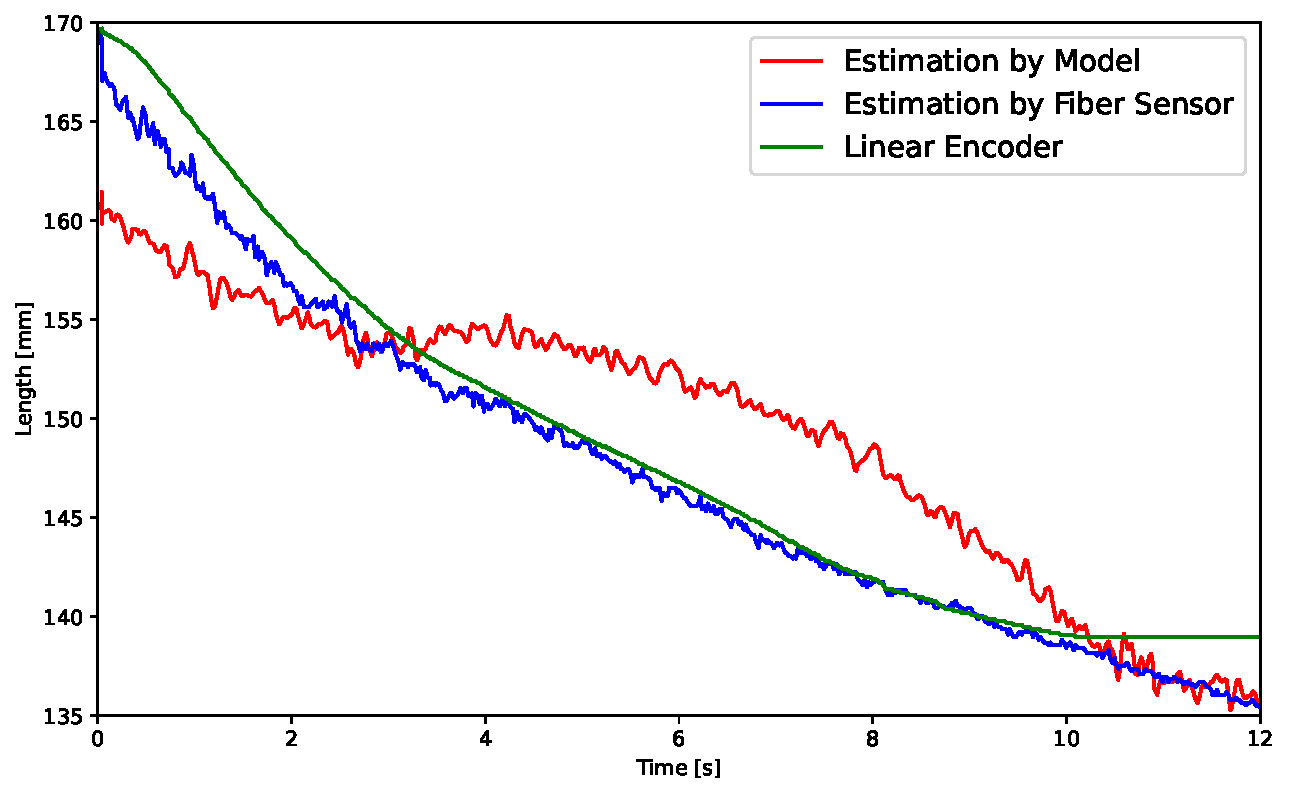
\includegraphics[width=\columnwidth]{fig/reaching_error.pdf} 
%         \caption{Relationship between Pressure and Natural Length}
%         \label{fig:length_pressure}
%         \vspace{1em} 
%         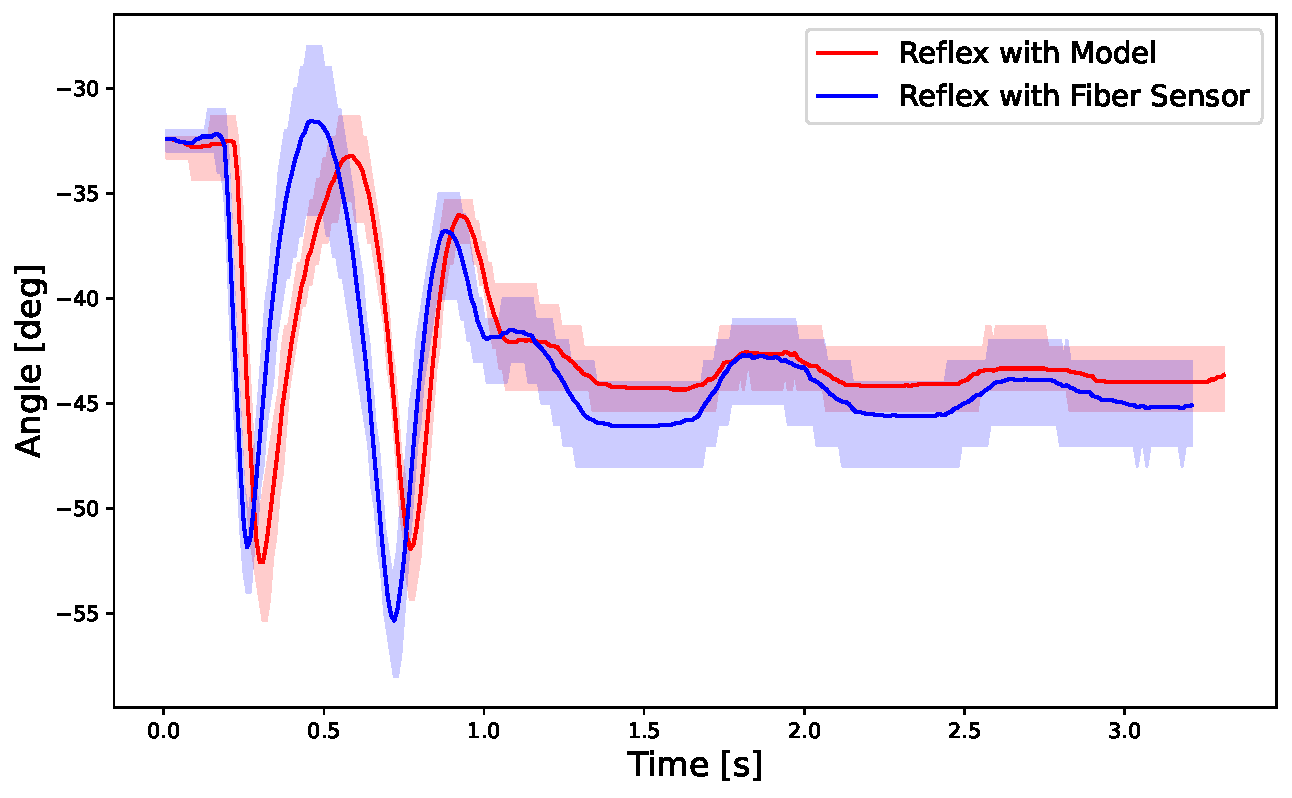
\includegraphics[width=\columnwidth]{fig/time_vs_angle_model_sensor.pdf}
%         \caption{Relationship between Force and Deformation at Each Pressure (PAM-B)}
%         \label{fig:pam_b_static1}
%     \end{minipage}
%     \hspace{0.05\textwidth} 
% \end{figure}

\begin{figure*}[t]
    \centering
    \begin{minipage}[H]{\textwidth} % 全幅を使用
        \begin{minipage}[H]{0.48\textwidth} % 左側の半分
            \centering
            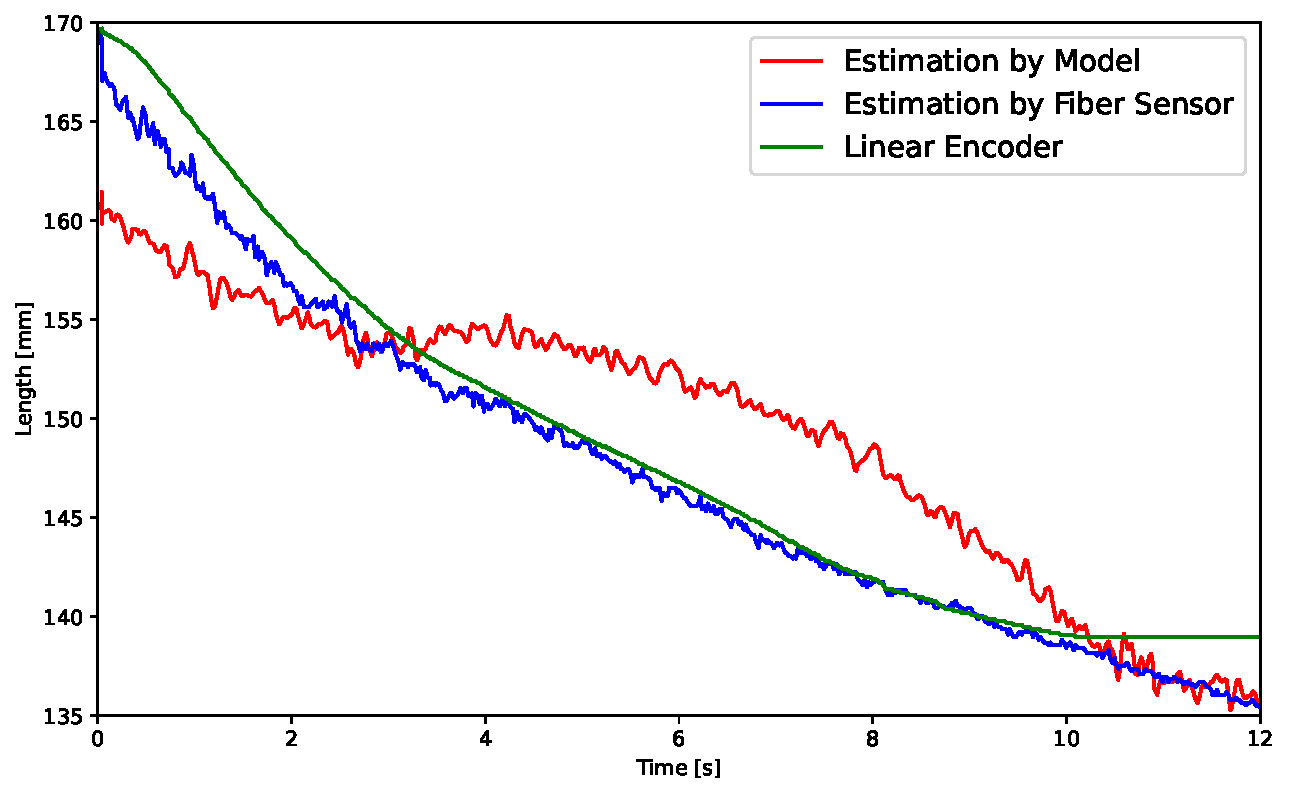
\includegraphics[width=\columnwidth]{fig/reaching_error.pdf}
            \caption{Length Estimation Error in Reaching Task}
            \label{fig:reaching_error}
            \vspace{1em}
            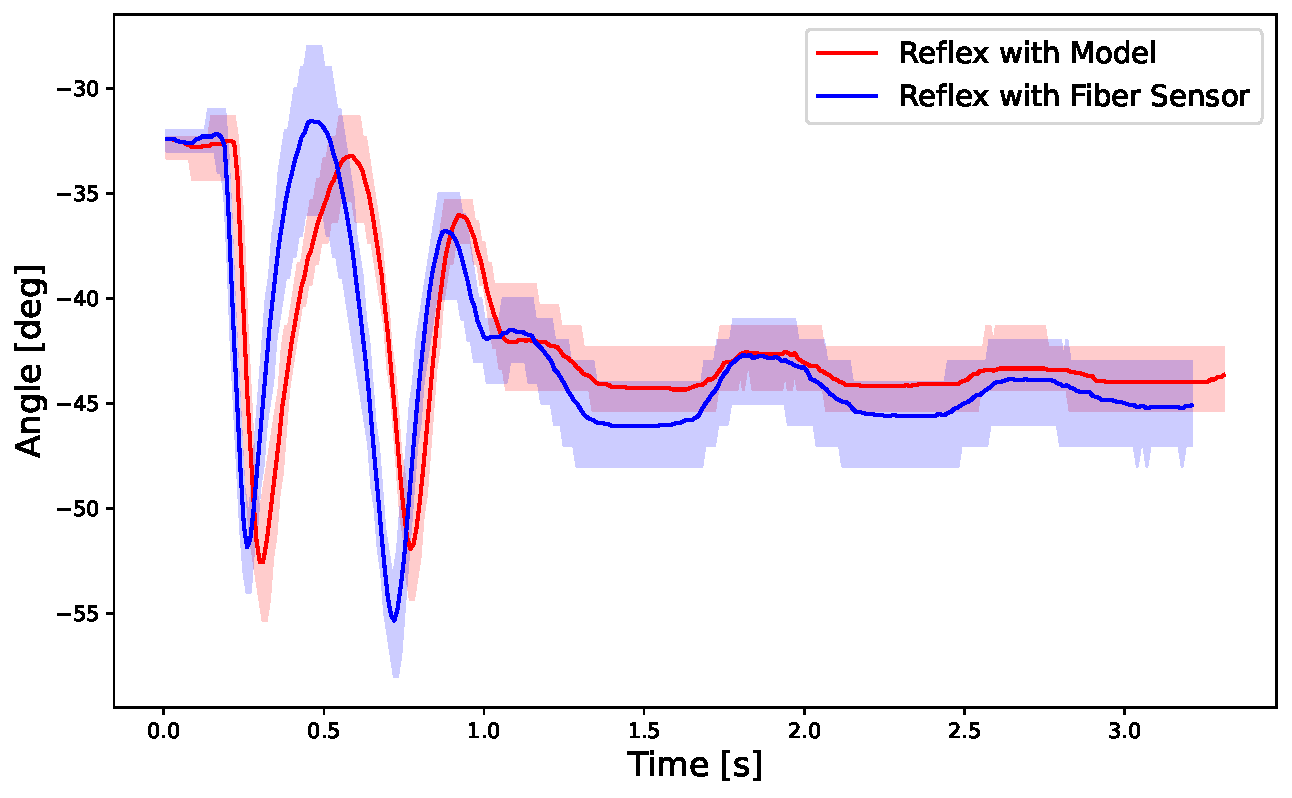
\includegraphics[width=\columnwidth]{fig/time_vs_angle_model_sensor.pdf}
            \caption{Comparison of Reflex Angles between Model and Fiber Sensor }
            \label{fig:reflex_angle}
        \end{minipage}
        \hfill
        \begin{minipage}[H]{0.48\textwidth} % 右側の半分
            \centering
            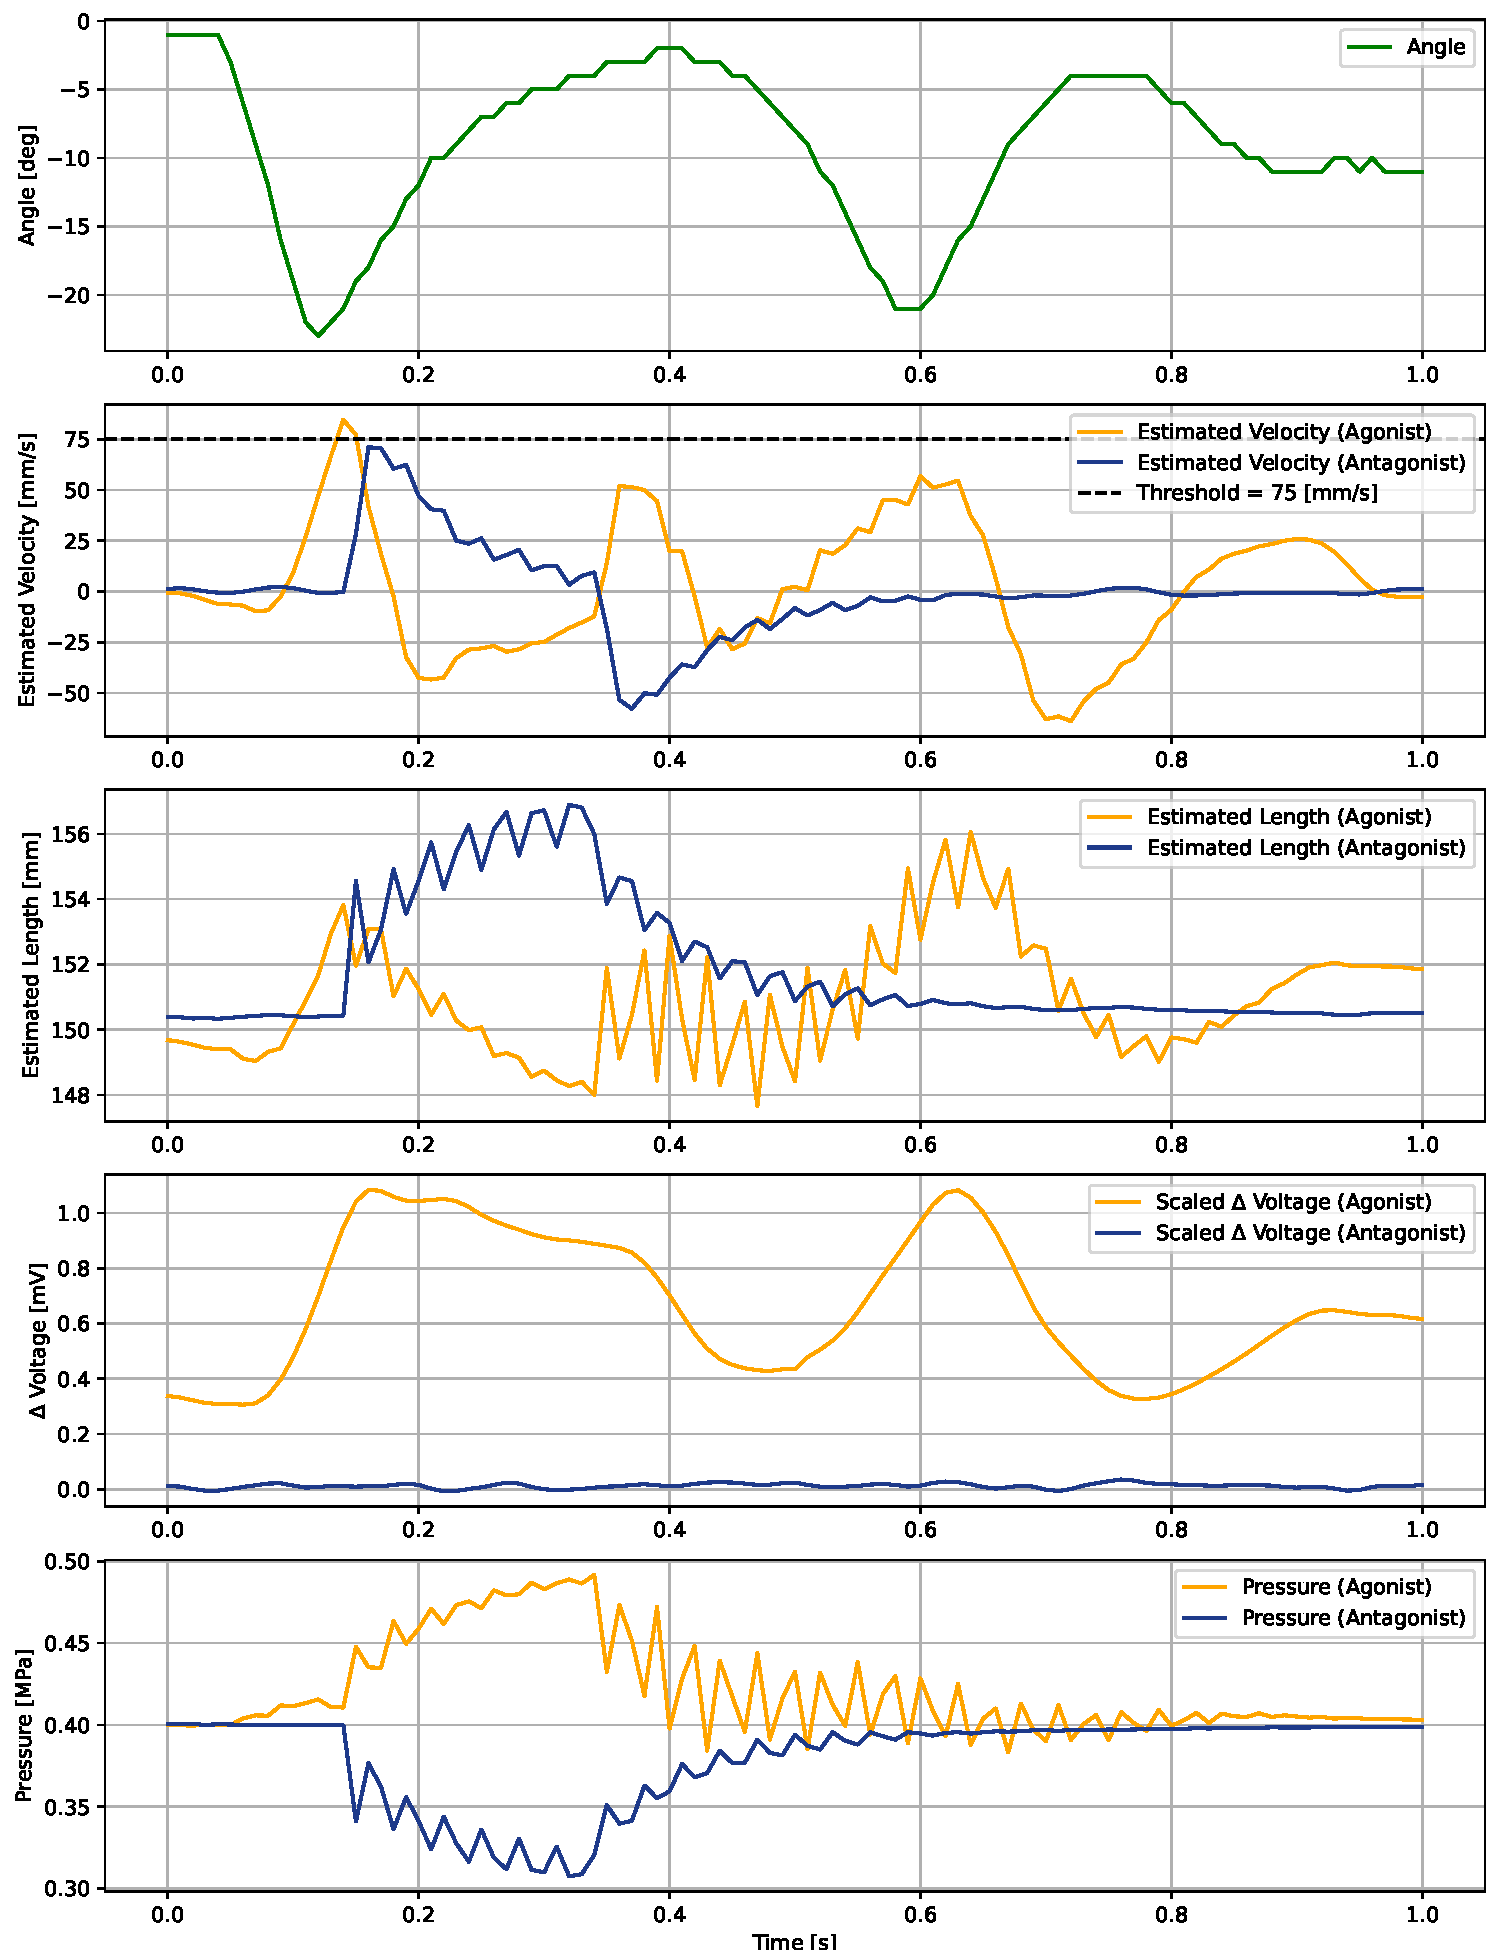
\includegraphics[width=\columnwidth]{fig/20240819_r20_reflex_all_plt.pdf}
            \caption{Dynamic Reflex Behavior of Agonist and Antagonist Muscles}
            \label{fig:reflex_all}
        \end{minipage}
    \end{minipage}
\end{figure*}

\noindent mechanism. If the parameters have to be switched depending on the situation, it would be difficult for the reflex mechanism to respond quickly to disturbances.
% Additionally, since the reflex mechanism is only required to detect sudden extension or contraction of the PAM, a minor decrease in precision is acceptable. 
% The reflex mechanism aims to reduce the computational load on the central control system, so the computational load ot the reflex mechanism itself must not be high. 
Musculoskeletal robots often carry microcomputers on their structures, so the employed length estimation method is desired to be simple for efficient operation given the limited computational resources.



% \begin{figure}[h]
%     \centering
%     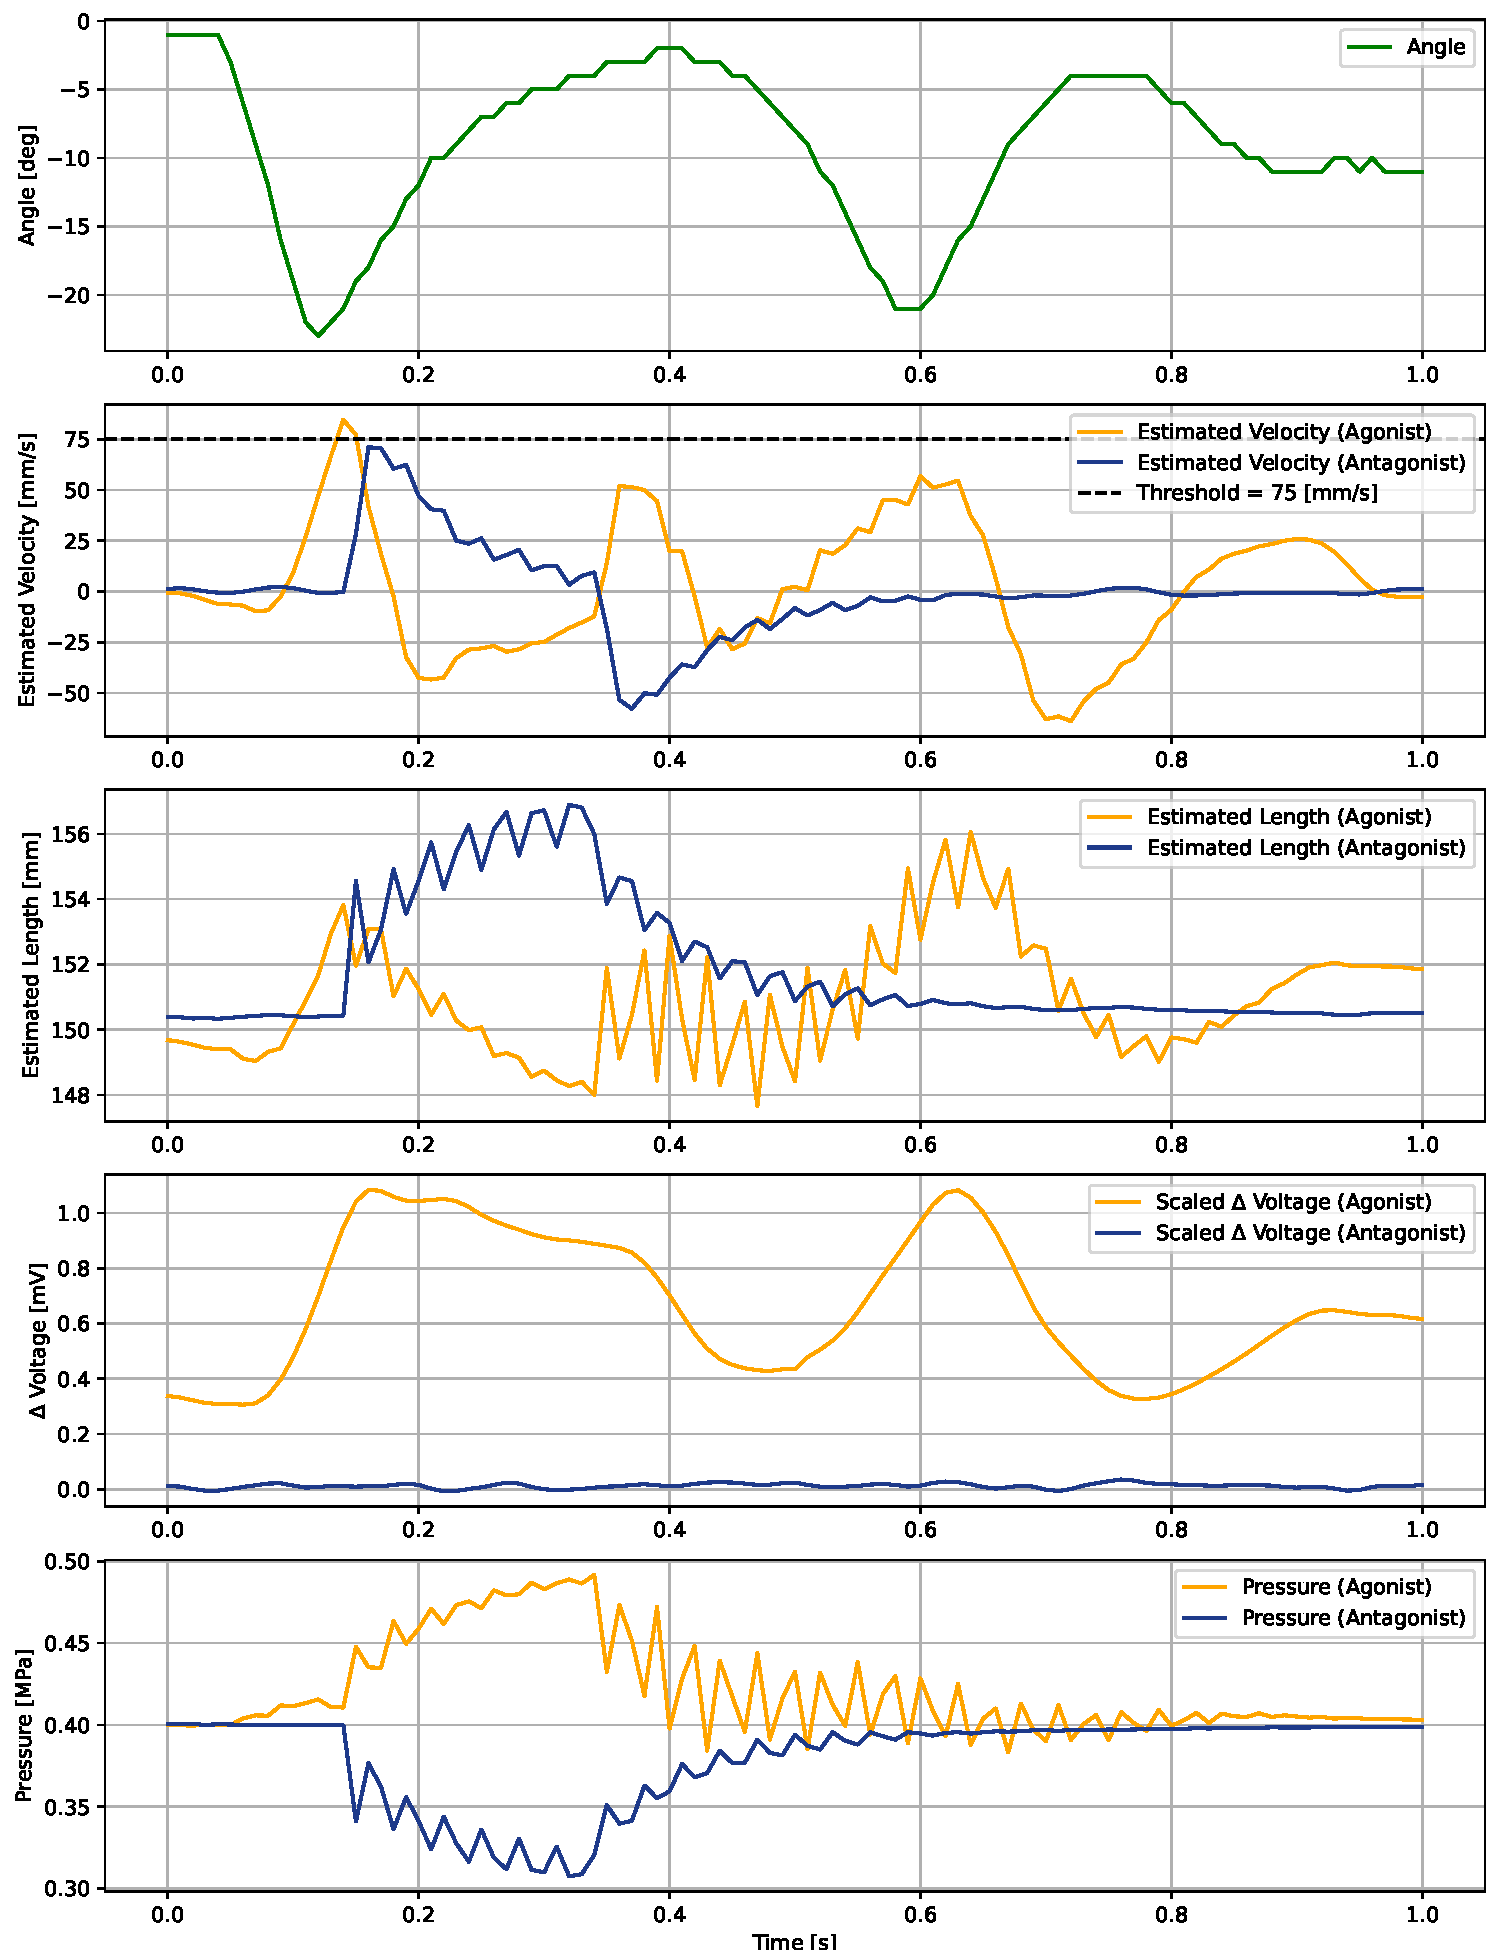
\includegraphics[width=\columnwidth]{fig/20240819_r20_reflex_all_plt.pdf}
%     \caption{Outline Diagram of Static Loading Experiment}
%     \label{fig:static_equipment}
%  \end{figure}

% \begin{figure*}[t] % figure* は twocolumn の場合、2カラム全体を使う
%     \centering
%     \begin{minipage}[t]{\columnwidth}
%         \centering
%         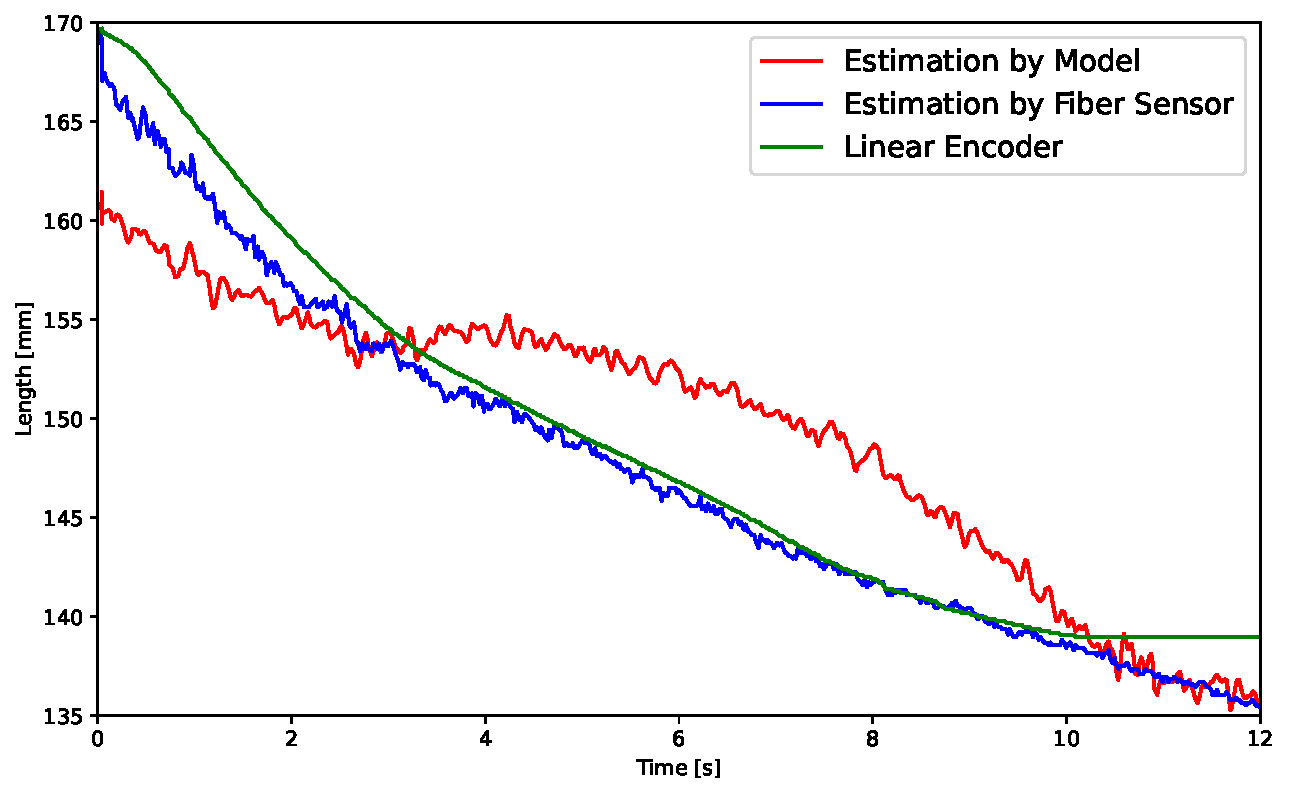
\includegraphics[width=\columnwidth]{fig/reaching_error.pdf}
%         \vspace{0.3cm}
%         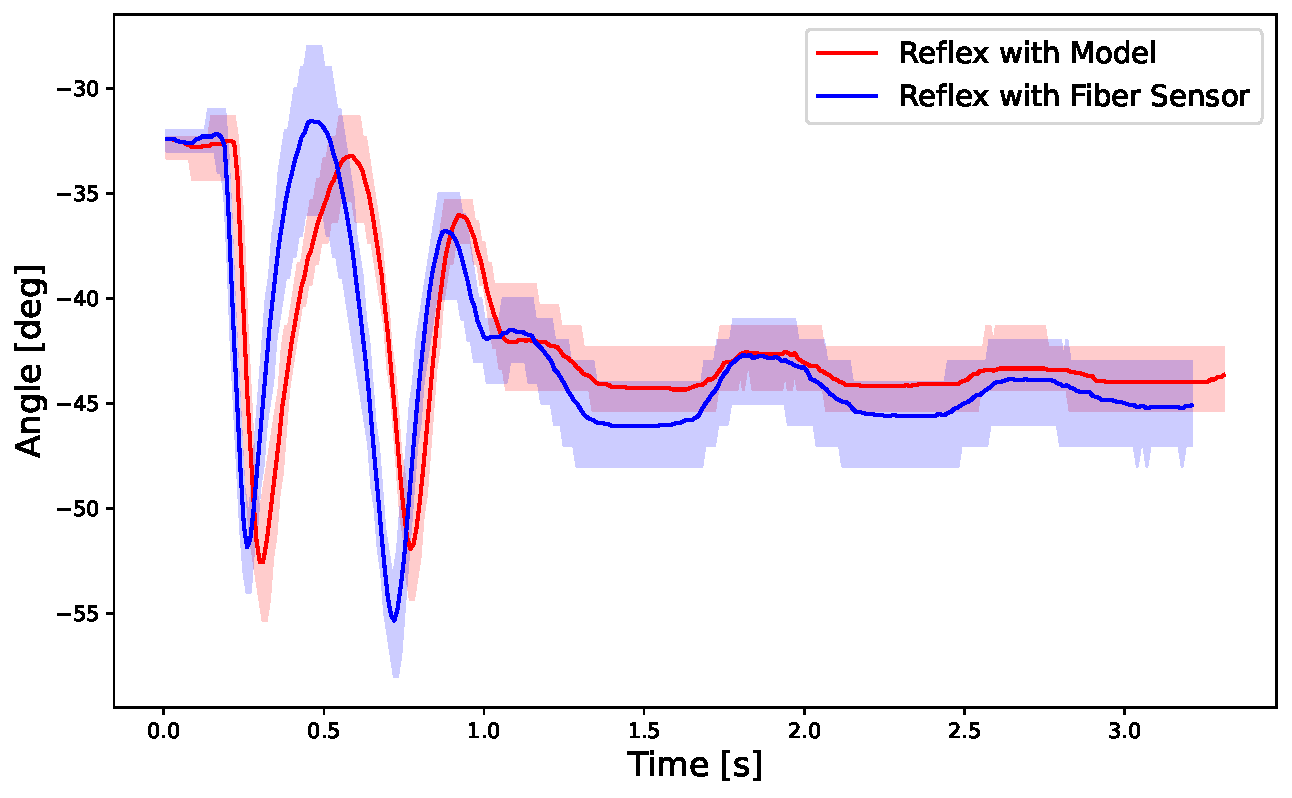
\includegraphics[width=\columnwidth]{fig/time_vs_angle_model_sensor.pdf}
%     \end{minipage}
%     \hfill
%     \begin{minipage}[t]{\columnwidth}
%         \centering
%         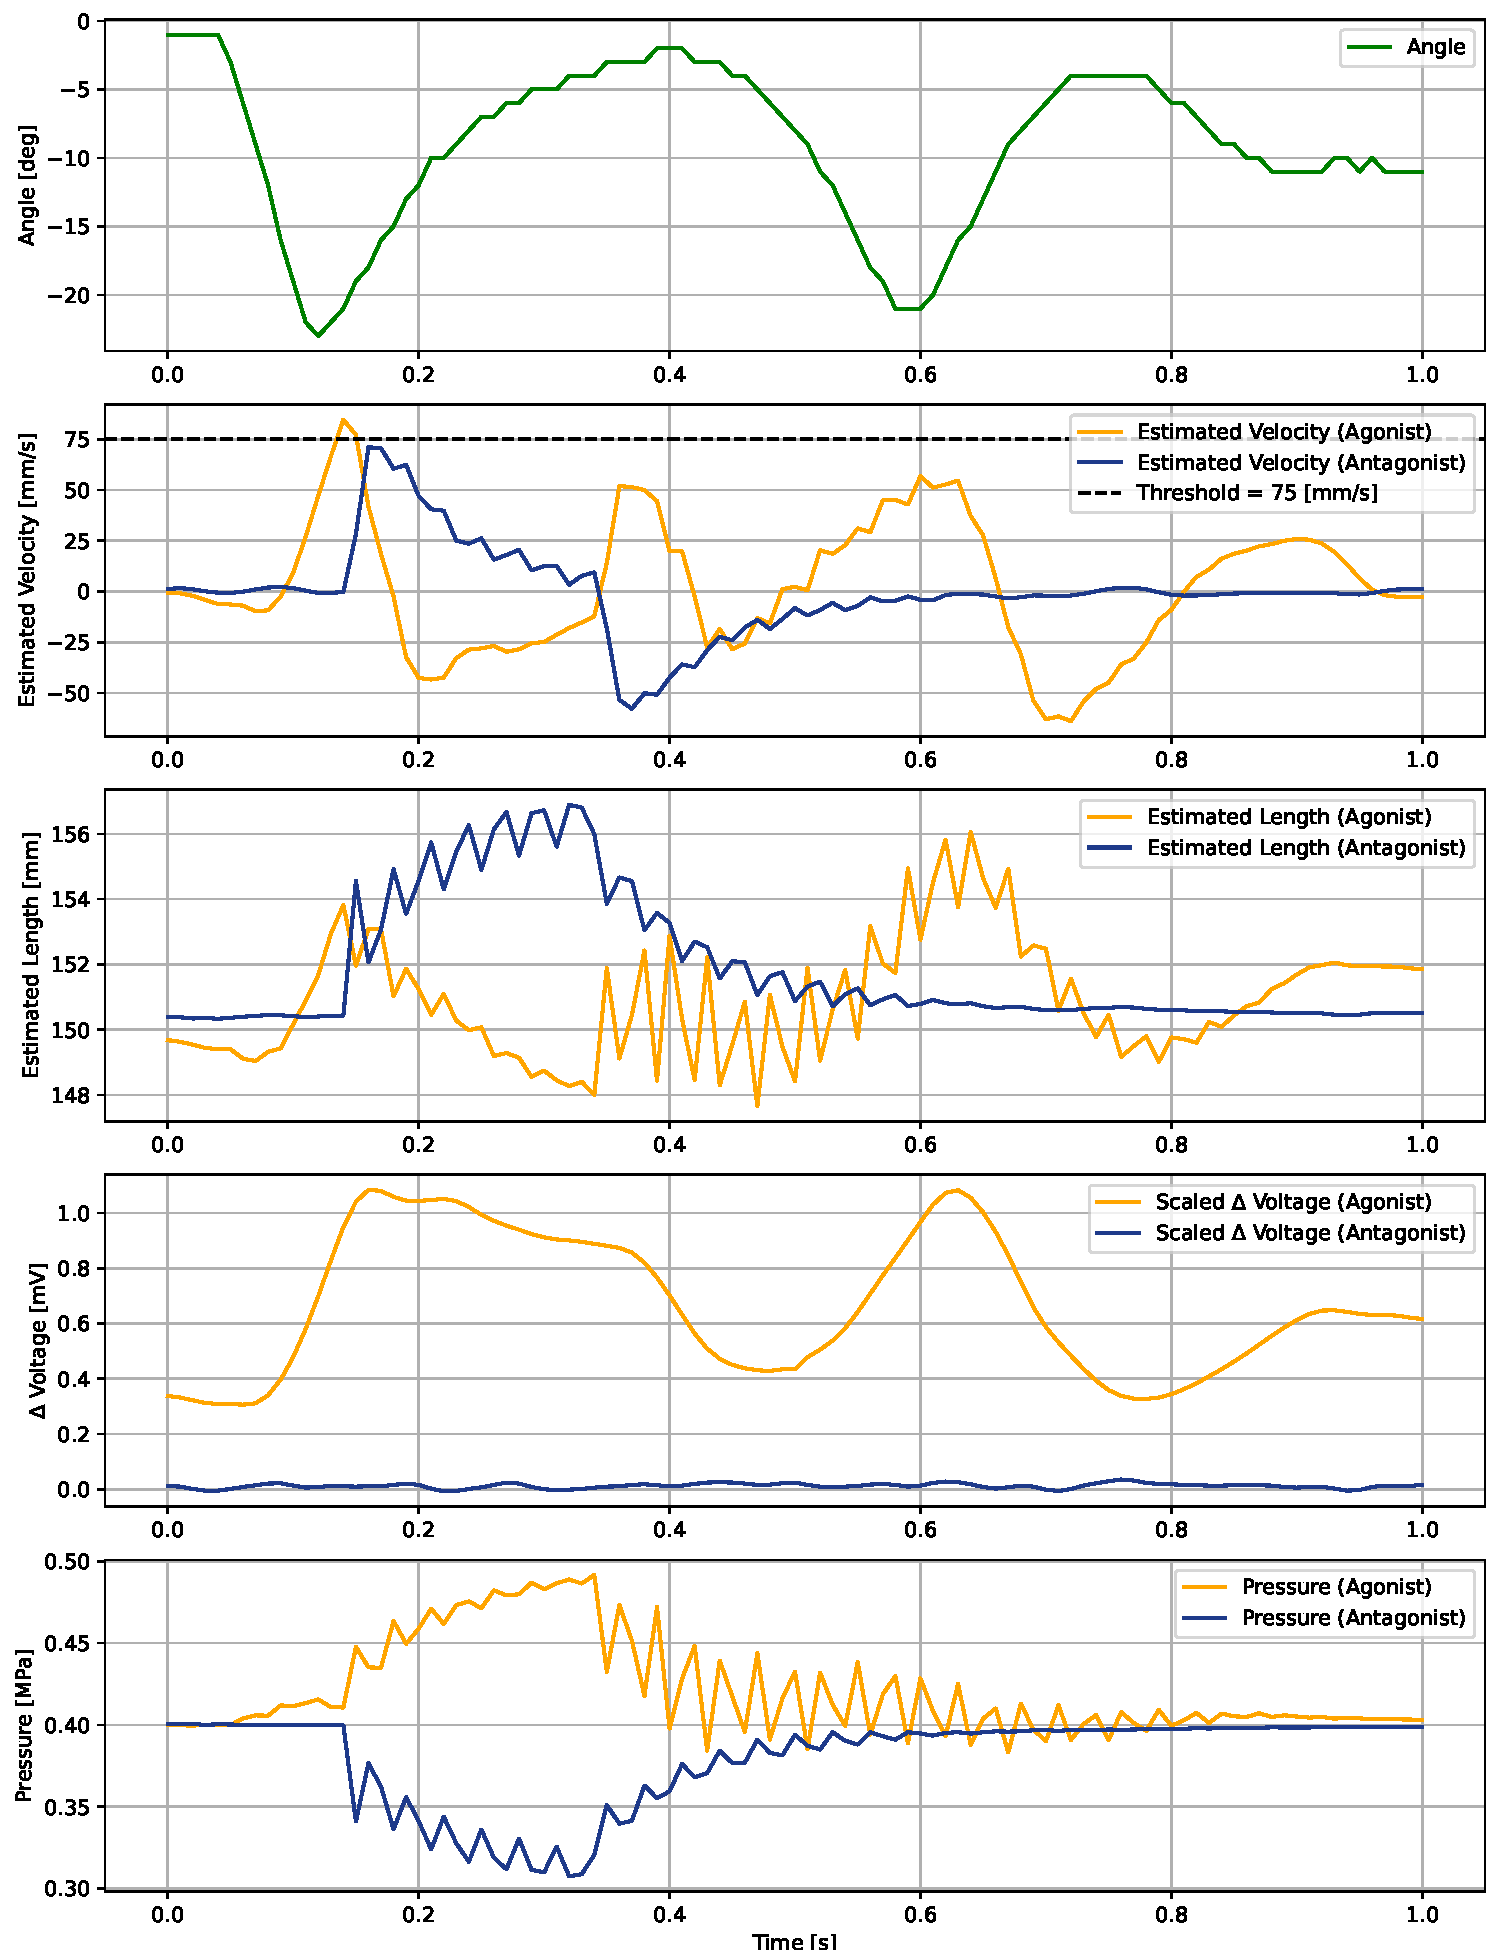
\includegraphics[width=\columnwidth]{fig/20240819_r20_reflex_all_plt.pdf}
%     \end{minipage}
%     \caption{a}
%     \label{fig:plots}
% \end{figure*}



\subsection{Reaching task}
\subsection{Stretch Reflex}

\newpage


% なお,WickramatungeらはPAMのヒステシスをモデルに反映させるために,推定パラメータ$a_i$を収縮時のパラメータ$a^c_i$と膨張時のパラメータ$a^e_i$に分けることを提案している.また,更に精度を向上させるために,低圧帯と高圧帯でもパラメータを使い分けることを提案している.本論文では,これらの提案を無視し,収縮・膨張を問わず全圧力範囲で同一のパラメータを用いることで,長さ推定の手法を単純化している.これは,本モデルによるPAMの長さ推定を反射機構に適用することを想定しているからである.推定パラメータを状況により切り替える必要があると,反射機構が外乱に迅速に反応することが困難になる.また,反射機構にはPAMの突然の伸長もしくは収縮を検知することだけが求められているので,PAMの精密な制御に求められるような高精度さは必要ないと考える.反射機構は中央制御系の計算負荷を軽減することを目的とするため,反射機構の計算負荷自体が高くてはならない.特に,筋骨格ロボットにはマイクロコンピュータを搭載することも多いため,計算資源の限られた環境での実行を考慮して,モデルを単純化している.
 


% To reduce the error in the length estimation, we expanded the spring constant in Equation (\ref{eq:model}) to a cubic polynomial of pressure $P$ and deformation $L_d$ and increased the number of the parameters as follows:

% \begin{equation}
% \label{eq:model_2d(1)}
% F = (b_5P^2 + b_4PL_d + b_3L^2_d + b_2P+b_1L_d+b_0)L_d
% \end{equation}

% Consequently, in some cases, the errors were actually increased as indicated in the third and fourth columns of Table \ref{tab:error}. This may be due to overfitting caused by an excessive increase in the parameters.
% In order to improve the accuracy of length estimation while avoiding overfitting to errors, it is necessary to investigate the contribution of each term of the spring constants in equations (\ref{eq:model}) and (\ref{eq:model_3d}) to fitting and to verify whether each term should be removed or added. The effect of each term during length estimation also depends on the reliability of a pressure sensor and a force sensor. For example, if the error of a pressure sensor is very small, adding the term $a_4P^3$ to the spring constants in equation (\ref{eq:model}) may reduce the error.

% \begin{equation}
%     \label{eq:model_3d}
%     F = (c_4P^3+c_3P^2L_d+c_2PL^2_d+c_1L^2_d+c_0)L_d
% \end{equation}
    
% 提案モデルによる長さ推定の誤差を低減しようと,(\ref{eq:model})式のバネ定数を
% \begin{equation}
% \label{eq:model_3d}
% F = (a_4P^3 + a_3P^2L_d + a_2PL^2_s + a_1L_d^3 +a_0)L_d
% \end{equation}
% のように,圧力$P$と変形量$L_d$の三次式にし,推定パラメータの数を増やした.
% その結果,表\ref{tab:error}の第4列および第5列に示すように,かえって誤差を増大させる場合があった.
% この原因として,過剰に推定パラメータを増やしたことで,誤差に対してオーバーフィティングするようになったことが考えられる.
% 誤差に対するオーバーフィッティングを防ぎつつ,長さ推定の精度を上げるには,
% (\ref{eq:model})式および(\ref{eq:model_3d})式のバネ定数の各項のフィッティングへの寄与を一つづつ調査し,
% 各項を削除もしくは追加するかを検証する必要がある.
% 長さ推定時の各項の効果には,圧力センサや力センサの信頼性も影響する.
% 例えば,圧力センサの誤差が非常に小さい場合,(\ref{eq:model})式のバネ定数に$a_4P^3$の項のみ追加すれば,
% 長さ推定の誤差が低減される可能性がある.

% \begin{table}[h]
%     \centering
%     \caption{Maximum error and root mean squared \\percentage error of dynamic length estimation }
%     \resizebox{\columnwidth}{!}{
%         \begin{tabular}{c|ccccccc}
%             \hline
%             PAM & \begin{tabular}[c]{@{}c@{}}Maximum Error[$\%$]\\(Eq.(\ref{eq:model})) \end{tabular} & \begin{tabular}[c]{@{}c@{}}Root Mean\\Squared Error[$\%$]\\(Eq.(\ref{eq:model})) \end{tabular} & \begin{tabular}[c]{@{}c@{}}Maximum Error[$\%$]\\(Eq.(\ref{eq:model_2d(1)})) \end{tabular} & \begin{tabular}[c]{@{}c@{}}Root Mean\\Squared Error[$\%$]\\(Eq.(\ref{eq:model_2d(1)})) \end{tabular}&\begin{tabular}[c]{@{}c@{}}Maximum Error[$\%$]\\(Eq.(\ref{eq:model_3d})) \end{tabular}&\begin{tabular}[c]{@{}c@{}}Root Mean\\Squared Error[$\%$]\\(Eq.(\ref{eq:model_3d})) \end{tabular} \\
%             \hline \hline
%             A & 1.72&0.861&1.12&0.633&1.22&0.516&\\
%             B & 1.19&0.653 &0.773&0.353&1.41&0.484&\\
%             C & 1.18&0.683&1.01&0.548&0.951&0.500&\\
%             D & 1.65 & 0.846 &0.755& 0.435&1.99&0.606&\\
%             \hline
%         \end{tabular}
%     }
%     \label{tab:error}
% \end{table}




 \footnotesize
% % \bibliographystyle{IEEEconf}
% \bibliography{bookmark}
% \bibliography{bookmark}

\begin{thebibliography}{99}

    \bibitem{rus_design_2015} D. Rus and M. T. Tolley, "Design, Fabrication and Control of Soft Robots", \textit{Nature}, vol. 521, pp. 467--475, 2015.
    
    \bibitem{Compac} H. Sato, K. Uchiyama, Y. Mano, F. Ito, S. Kurumaya, M. Okui, Y. Yamada, and T. Nakamura, "Development of a Compact Pneumatic Valve Using Rotational Motion for a Pneumatically Driven Mobile Robot With Periodic Motion in a Pipe", \textit{IEEE Access}, vol. 9, pp. 165271--165285, 2021.
    
    % \bibitem{polygerinos_soft_2015} P. Polygerinos, Z. Wang, K. C. Galloway, R. J. Wood, and C. J. Walsh, "Soft Robotic Glove for Combined Assistance and At-Home Rehabilitation", \textit{Robotics and Autonomous Systems}, vol. 73, pp. 135--143, 2015.
    %6ページ超えたので、スペース節約のために省略
    
    \bibitem{hosoda} K. Hosoda, S. Sekimoto, Y. Nishigori, S. Takamuku, and S. Ikemoto, "Anthropomorphic Muscular–Skeletal Robotic Upper Limb for Understanding Embodied Intelligence", \textit{Advanced Robotics}, vol. 26, no. 7, pp. 729--744, 2012.
    
    \bibitem{marchese_autonomous} A. D. Marchese, C. D. Onal, and D. Rus, "Autonomous Soft Robotic Fish Capable of Escape Maneuvers Using Fluidic Elastomer Actuators", \textit{Soft Robotics}, vol. 1, no. 1, pp. 75--87, 2014.
    
    \bibitem{mirvakili_artificial} S. M. Mirvakili and I. W. Hunter, "Artificial Muscles: Mechanisms, Applications, and Challenges", \textit{Advanced Materials}, vol. 30, no. 6, 2018.
    
    \bibitem{Dynamic} D. B. Reynolds, D. W. Repperger, C. A. Phillips, and G. Bandry, "Modeling the Dynamic Characteristics of Pneumatic Muscle", \textit{Annals of Biomedical Engineering}, vol. 31, no. 3, pp. 310--317, 2003.
    
    \bibitem{SDCharacteristics} C.-P. Chou and B. Hannaford, "Static and Dynamic Characteristics of McKibben Pneumatic Artificial Muscles",\textit{Proceedings of the 1994 IEEE International Conference on Robotics and Automation}, pp. 281--286, IEEE Comput. Soc. Press, 1994.
    
    \bibitem{ashwin_survey_2018} K. P. Ashwin and A. Ghosal, "A Survey on Static Modeling of Miniaturized Pneumatic Artificial Muscles With New Model and Experimental Results", \textit{Applied Mechanics Reviews}, vol. 70, no. 4, 2018.
    
    \bibitem{takahashi} R. Takahashi, Y. Wang, J. Wang, Y. Jiang, and K. Hosoda, "Implementation of Basic Reflex Functions on Musculoskeletal Robots Driven by Pneumatic Artificial Muscles",\textit{IEEE Robotics and Automation Letters}, vol. 8, no. 4, pp. 1920--1926, 2023.
    
    \bibitem{kandel} E. R. Kandel, J. H. Schwartz, T. M. Jessell, S. Siegelbaum, A. J. Hudspeth, S. Mack et al., "Principles of Neural Science", McGraw-Hill, vol. 4, 2000.
    
    \bibitem{nakajima} R. Sakurai, M. Nishida, H. Sakurai, Y. Wakao, N. Akashi, Y. Kuniyoshi, Y. Minami, and K. Nakajima, "Emulating a Sensor Using Soft Material Dynamics: A Reservoir Computing Approach to Pneumatic Artificial Muscle", \textit{2020 3rd IEEE International Conference on Soft Robotics (RoboSoft)}, pp. 710--717, 2020.
    
    \bibitem{motion} T. Nozaki and T. Noritsugu, "Motion Analysis of McKibben Type Pneumatic Rubber Artificial Muscle with Finite Element Method", \textit{International Journal of Automation Technology}, vol. 8, pp. 147--158, 2014.
    
    \bibitem{spring} K. C. Wickramatunge and T. Leephakpreeda, "Empirical Modeling of Dynamic Behaviors of Pneumatic Artificial Muscle Actuators", \textit{ISA Transactions}, vol. 52, no. 6, pp. 825--834, 2013.
    
    \bibitem{chouMeasurementModelingMcKibben1996} C.-P. Chou and B. Hannaford, "Measurement and Modeling of McKibben Pneumatic Artificial Muscles", \textit{IEEE Transactions on Robotics and Automation}, vol. 12, no. 1, pp. 90--102, 1996.
    
    \bibitem{ModelingControl} B. Tondu and P. Lopez, "Modeling and Control of McKibben Artificial Muscle Robot Actuators", \textit{IEEE Control Systems}, vol. 20, no. 2, pp. 15--38, 2000.
    
    \bibitem{Comparison} W. F. Carlo Ferraresi and A. Manuello, "Flexible Pneumatic Actuators: A Comparison between The McKibben and the Straight Fibres Muscles", \textit{Journal of Robotics and Mechatronics}, vol. 13, no. 1, pp. 56--63, 2001.

    \bibitem{fiber} A. Hitzmann, Y. Wang, T. Kessler, and K. Hosoda, "Using conductive fabrics as inflation sensors for pneumatic artificial muscles", \textit{Advanced Robotics}, pp. 1--17, 2021.


    \bibitem{wheatstone} K. Hoffmann, "Applying the Wheatstone Bridge Circuit," HMB Germany, 1974.

    \bibitem{spindle} C. C. Hunt and S. W. Kuffler, "Stretch Receptor Discharges during Muscle Contraction," \textit{The Journal of Physiology}, vol. 113, no. 2-3, pp. 298--315, 1951.


  
    
    \end{thebibliography}
    

    

\end{document}
